\documentclass[12pt]{memoir}
\setcounter{tocdepth}{4}
\setcounter{secnumdepth}{3} 
\usepackage[dvipsnames]{xcolor}
\usepackage[utf8]{inputenc}
\usepackage[margin=1in]{geometry}
\usepackage{fancyhdr}
\usepackage{url}
\usepackage{pdfpages}
\raggedbottom
% \usepackage{biblatex}
\usepackage[
backend=biber,
style=alphabetic,
sorting=ynt
]{biblatex}
\addbibresource{bibliography.bib}

% Images and figure packages
\usepackage{float}
\usepackage{svg}
\usepackage{subcaption}

% Math packages
\usepackage{amssymb}
%\usepackage[cal=boondoxo]{mathalfa}
\usepackage{amsmath}
\usepackage{empheq}
\usepackage{thmtools}
\usepackage{mathtools}
\newtheorem{definition}{Definition}
\newtheorem{theorem}{Theorem}

\declaretheorem[sibling=definition, shaded={rulecolor=black, rulewidth=0.6pt, bgcolor={rgb}{1,1,1}},name=Definition]{boxeddef}
\declaretheorem[sibling=theorem, shaded={rulecolor=black, rulewidth=0.6pt, bgcolor={rgb}{1,1,1}},name=Theorem]{boxedthm}



\usepackage{hyperref}
\hypersetup{
    colorlinks=true,
    linkcolor=blue,
    filecolor=magenta,      
    urlcolor=cyan,
    citecolor=Green,
    pdftitle={Thesis - Danila Mokeev},
    pdfpagemode=FullScreen,
}
\usepackage{underscore}
\usepackage{braket}
\usepackage{afterpage}

% algorithms
\usepackage[linesnumbered,ruled]{algorithm2e}

\setlength\parindent{0pt}

% Commands/shortcuts
% example def of command
% \newcommand{\plusbinomial}[3][2]{(#2 + #3)^#1}
% 3 parameters, with 2 as a default value for #1
\newcommand{\tr}{\text{tr}}
\newcommand{\Tr}{\text{Tr}}
\newcommand{\mb}{\mathbf}
\newcommand{\bsy}{\boldsymbol}
\newcommand{\tb}{\textbf}
\newcommand{\ti}{\textit}
\newcommand{\btheta}{\boldsymbol{\theta}}
\newcommand{\brho}{\boldsymbol{\rho}}
\newcommand{\nmeasn}[1]{$n_{\text{meas}}=#1$}
\newcommand{\nitern}[1]{$n_{\text{iter}}=#1$}
\newcommand{\nburninn}[1]{$n_{\text{burnin}}=#1$}
\newcommand{\rhorankn}[1]{\text{rank}$(\rho)=#1$}
\newcommand{\nmeas}[0]{$n_{\text{meas}} $ }
\newcommand{\niter}[0]{$n_{\text{iter}} $ }
\newcommand{\nburnin}[0]{$n_{\text{burnin}} $ }
\newcommand{\rhorank}[0]{\text{rank}$(\rho) $ }
\title{Efficient sampling algorithms for Bayesian Quantum Tomography}
\author{Danila Mokeev}
\date{June 2024}

\begin{document}
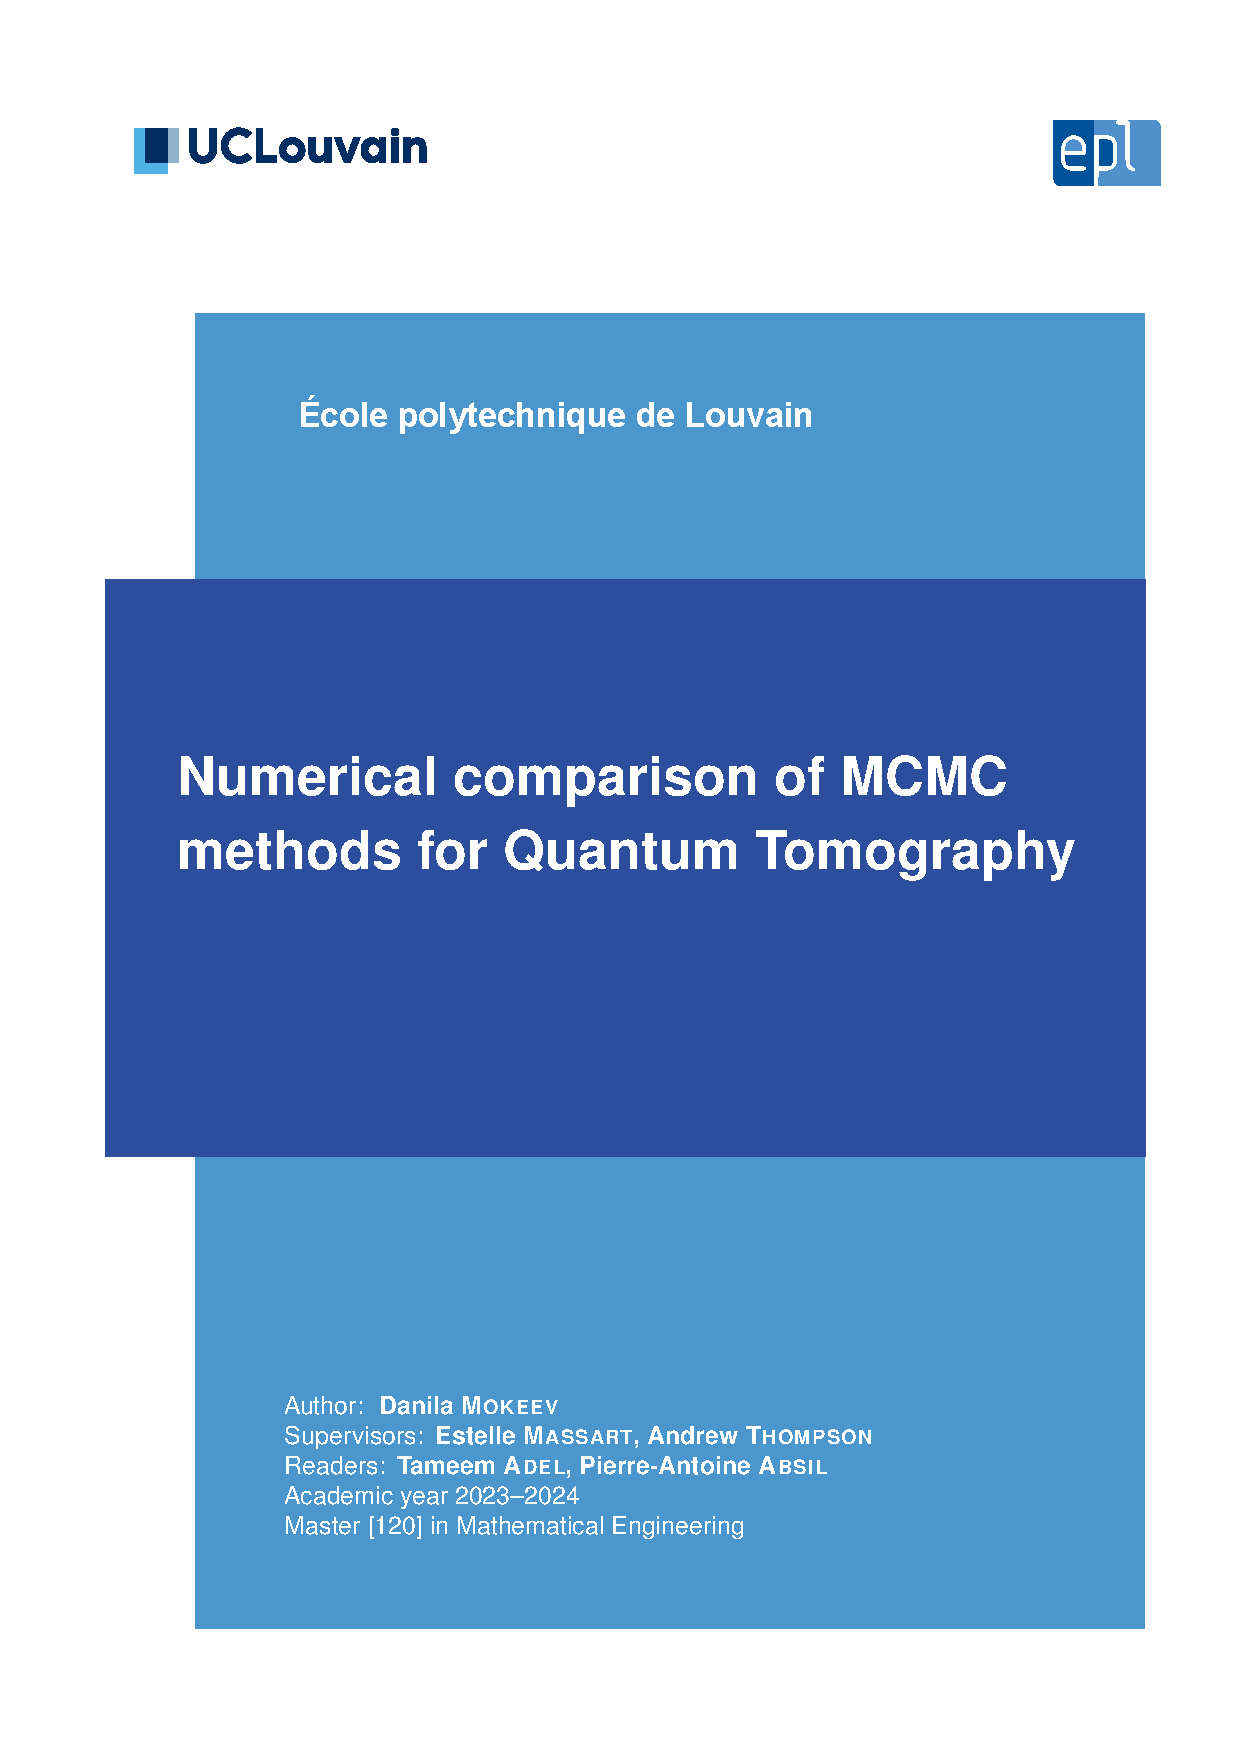
\includepdf[pages={1}]{cover/cover-danila-mokeev.pdf}

\chapter*{Acknowledgements}
I would like to thank Estelle Massart, Andrew Thompson and Tameem Adel for their help in the making of this thesis. Their guidance and great ideas were valuable in its success. I also want to thank Matthieu Génévriez for his help on making the Quantum Tomography section more rigorous, and researchers Pierre Alquier and The Tien Mai for providing the source code for the prob-estimator. Finally, I want to thank my family who supported me throughout the university years, and my friends, who made them more enjoyable.
\newpage

\tableofcontents*

\newpage

\chapter*{Abbreviations and symbols}
\addcontentsline{toc}{chapter}{\protect\numberline{}Abbreviations and symbols}
\begin{tabular}{p{0.2\linewidth} | p{0.8\linewidth}}
{MCMC} & Markov chain Monte Carlo\\
{POVM} & Positive Operator-Valued Measure\\
{MHS}  & Metropolis-Hastings with Student-t prior algorithm \\
{MHGS}  & Metropolis-Hastings with Gibbs with Student-t prior algorithm\\
$\ket{{\psi}}$ & Quantum state $\psi$ in the \ti{bra-ket} formulation\\
${M^\dagger}$ & Conjugate transponse of matrix $M$\\
$\braket{M}$ & Expected value of a matrix/operator $M$\\
${M\otimes N}$ & Kronecker product between matrices $M$ and $N$\\
${M \odot N}$ & Hadamard (element-wise) product between matrices $M$ and $N$\\
${U}(a,b)$ & Uniform distribution defined on the open interval $(a,b)$\\
$N(\mu, \sigma^2)$ & Normal distribution with mean $\mu$ and variance $\sigma^2$\\
$N(\boldsymbol{\mu},\boldsymbol{\Sigma})$ & Multivariate normal distribution with mean vector $\boldsymbol{\mu}$ and covariance matrix $\boldsymbol{\Sigma}$\\
$N(\mu, \sigma^2)^{d \times r}$& Matrix of size $d\times r $ where each entry is independently drawn from a univariate normal distribution with mean $\mu$ and variance $\sigma^2$ \\
$Gamma(\alpha,\beta)$ & Gamma distribution with shape $\alpha$ and rate $\beta$\\
$\mathcal{D}ir(\alpha_1,\dots,\alpha_d)$ & Dirichlet distribution with concentration parameters $\alpha_1,\dots,\alpha_d > 0$
\end{tabular}

\chapter{Introduction}

\section{Motivation}
%\addcontentsline{toc}{chapter}{\protect\numberline{}Motivation}
A fundamental problem in physics is the reconstruction of the state of a system given measurements describing it. In classical mechanics, this is, at least in theory, always possible due to the deterministic nature of the system. This allows one to make multiple measurements on a system, usually the position and momentum, to exactly determine its state. In Quantum Mechanics, however, the situation is very different: measuring the system disturbs it (in Quantum Mechanics we talk about wavefunction collapse), making it impossible to gain more information by repeating measurements. We are also fundamentally limited by what we can measure: the Heisenberg uncertainty principle only allows the measurement of either the position or the momentum, but not both at the same time. Finally, the no-cloning theorem also forbids the system to be copied right before the measurement unless we know the state of the system.\medbreak

\textit{Quantum Tomography} or \textit{Quantum State Tomography} is a process that allows to reconstruct the state of a system in the context of Quantum Mechanics. It tackles the previously described issues by replicating the initial state of the system multiple times, and then measuring once each replica. Note that there is a subtle difference between copying the system and preparing multiple systems with the same steps, as the latter does \textit{not} require any knowledge about the state, only the \textit{steps} necessary to produce it.\medbreak

The term ``tomography" means ``to describe an object based on sections, slices" \cite{wiki:tomography}. Many types of tomographies exist and are used in very diverse environments, with notable examples in medical applications, such as Computed Tomography (CT) or Magnetic Resonance Imaging (MRI). Quantum Tomography works in a similar way: we use a set of slices (observables), each of them probing a particular aspect of that state, to reconstruct the quantum state through a tomographic process. An intuitive analogy is the process of shining light on each side of a 3D object, and reconstructing that object from the obtained shadows. This results in an inverse problem, whereby starting from partial and noisy data (and in this case fundamentally probabilistic), we can obtain the true state of the system.


\section{Quantum Tomography} \label{introduction:quantum-tomography}

As previously described, the goal of Quantum Tomography is the reconstruction of the system state based on measurements. All of this system information is stored in a matrix, called the \textit{density matrix} $\rho \in \mathbb{C}^{d \times d}$, with $d = 2^n$ and $n$ the number of qubits. Due to the physical properties of the system, this matrix is Hermitian ($\rho = \rho^{\dagger}$), positive semi-definite ($\rho > 0$) and satisfying $\tr(\rho) = 1$. The rank of the matrix also has importance: pure states are of rank 1, while mixed states are of any rank between 2 and $d$. A pure state is described by the wavefunction, which is usually represented by a vector (or equivalently a rank-1 matrix), of potentially infinite dimension . Mixed states, on the other hand, are a generalization of pure states and are represented by a density matrix. They correspond to a probabilistic mixture of pure states. It is important to note that physicists are mostly interested in density matrices of low rank.\medbreak

Quantum Tomography is based on Born's rule, which links a projective measurement $P_m$ associated to an \textit{observable} $O$ to the probability $p(m)$ of obtaining the associated eigenvalue $m$ given a density matrix $\rho$. This can generally be written as 
\begin{equation}
    p(m) = \tr(\rho P_m)
\end{equation}
By repeating the measurement on many different but identically prepared systems for each observable, we are able to obtain statistically significant estimates for $p(m)$, which combined with the projectors $P_m$, allows us to estimate the density matrix with any appropriate method.
\section{Overview of existing methods}\label{section:litterature-review}
We first provide in \ref{table:methods-comp} a summary of existing methods with the papers using them, followed by a more detailed explanation below.  

\begin{table}[H]

\begin{center}
    \begin{tabular}{|c|c|}
        \hline
        Method & Papers \\\hline\hline
        Inversion & \cite{meth:linear-inversion:vogel-risken, meth:linear-inversion:RMH, meth:linear-inversion:alquier} \\\hline
        Pauli basis expansion & \cite{Cai-2016}\\\hline
        Maximum Likelihood & \cite{Guta20,meth:ML:BDP,meth:ML:JKMW,meth:ML:Lvovsky,meth:ML:Blume-Kohout,meth:ML:Suzuki,meth:ML:Hradil2004} \\\hline
        Compressed Sensing & \cite{meth:CS:GLFSBE10,meth:CS:Gross-2011, meth:CS:Flammia-2012,meth:CS:Koltchinskii-2011}\\\hline
        Sampling based & \cite{meth:bayesian:smc:Ferrie-2014,meth:bayesian:smc:Kueng-2015, meth:bayesian:smc:Granade_2016,meth:bayesian:sis:Kravtsov-2013}\\\hline
        Metropolis-Hastings based & \cite{MA17,Mai22,LLJL20, meth:bayesian:mh:Cotter2013, meth:bayesian:mh:Blume-Kohout-2010}\\\hline
        Langevin & \cite{meth:bayesian:Langevin:ACMT2024}\\\hline
    \end{tabular}
\end{center}
\caption{Overview of existing methods with associated papers}
\label{table:methods-comp}
\end{table}


Well-established methods exist to approximate $\rho$. We can split the existing methods into 5 main categories: inversion, Pauli basis expansion, Maximum Likelihood, Compressed sensing and finally Bayesian methods, which are mostly sampling-based algorithms.\medbreak

Inversion methods are very simple, as they directly rely on the Born rule: $\hat \rho$ is computed by solving the linear system of equations defined by 
\begin{equation*} \label{eq:inversion-method}
        \forall \mb a \in \mathcal{A},\forall \mb s \in \mathcal{S}: \, \hat p_{\mb a, \mb s} = \tr(\hat \rho P^{\mb a}_{\mb s})
\end{equation*}
where $\mathcal{A}$ denotes the set of indices for observables, $\mathcal{S}$ the set of indices for projective measurements, $\hat p_{\mb a,\mb s}$ the empirical probability and $P^{\mb a}_{\mb s}$ the projection operator. This approach was introduced in \cite{meth:linear-inversion:vogel-risken}, and then used in \cite{meth:linear-inversion:RMH}, but also in \cite{meth:linear-inversion:alquier}, where they additionally use a rank penalization term. This method is easy to understand, however, it returns a matrix $\hat \rho$ which does not satisfy the properties of a density matrix.\medbreak
%and requires the set of observables to be tomographically complete, which is usually the case but limits us, for example, to run any ablation studies related to the number of observables.
% \begin{equation}
%     \hat p_{a,s} = \tr(\hat \rho \cdot P^{a,s})
% \end{equation}
A second approach, introduced in \cite{Cai-2016}, works by estimating the coefficients in the Pauli basis expansion. Indeed, as the observables of interest we use in Quantum Tomography are the Kronecker product of Pauli matrices (which are usually called $\{\sigma_x, \sigma_y, \sigma_z\} \in \mathbb{C}^{2\times 2}$), we can also approximate $\rho$ using the resulting observable as an element of a base. If we have $\mathcal{B} = \{\sigma_b = \sigma_{b_1} \otimes \dots \otimes \sigma_{b_n}, b \in \{I,x,y,z\}^n\}$, then the density matrix $\rho$ can be approximated as 
\begin{equation}
    \rho = \sum_{b\in\{I,x,y,z\}^n} \rho_b \sigma_b
\end{equation}
In the case of \cite{Cai-2016}, the coefficients $\rho_b$ are estimated using an average of the measured eigenvalues with each observable.\medbreak

Another common approach used by many \cite{Guta20,meth:ML:BDP,meth:ML:JKMW,meth:ML:Lvovsky,meth:ML:Blume-Kohout,meth:ML:Suzuki,meth:ML:Hradil2004} is Maximum Likelihood (ML) estimation, which tries to maximize an objective function $\mathcal{L}$ to find the best $\rho$ which matches the data. A possible loss function could be 
\begin{equation}
\mathcal{L}(\rho ; \mb{D}) \propto \prod_{\mb a \in \mathcal{A}} \prod_{\mb s \in \mathcal{S}}\left[\tr\left(\rho P_{\mb{s}}^{\mb{a}}\right)\right]^{n_{{\mb a}, {\mb s}}},
\end{equation}
where $n_{\mb a,\mb s}$ is the number of occurences of $\mb s$ in measurements by $\mb a$. The density matrix is calculated as 
\begin{equation}
    \hat \rho_{\text{ML}} = \text{argmin}_{\rho} \;\mathcal{L}(\rho;\mb{D})
\end{equation}
A downside however often mentioned for this method is the cost, notably for $n\geq10$.
\medbreak

There is also a certain number of papers \cite{meth:CS:GLFSBE10,meth:CS:Gross-2011, meth:CS:Flammia-2012,meth:CS:Koltchinskii-2011} which treat the problem of solving \ref{eq:inversion-method} as a pure optimization problem, with the extra contraint that not all observables are available (compressed sensing). They are however less relevant to us, as we (mostly) consider to be in the complete measurement case.\medbreak

The methods described so far do not make any assumptions about the structure of $\rho$. They may enforce the properties of a density matrix, but not use the low-rank information, with the only exception being papers that include a rank regularization term in the loss function (such as \cite{meth:linear-inversion:alquier}). To tackle this issue, a good idea is to venture into Bayesian methods, which naturally define a \textit{prior} on $\rho$. They also have the advantage of providing a distribution over it, rather than a point estimate, as most optimization-based methods do. This gives us uncertainty quantification.\medbreak

Bayesian methods rely on \ti{Bayes} theorem, which states that given data $\mb{D}$, which in our case are the empirical probabilities $p_{\mb a, \mb s}$ and projectors $P^{\mb a}_{\mb s}$, and parameters $\theta$, in our case the density matrix $\rho$, we can calculate the posterior distribution $\pi(\rho|\mb{D})$:
\begin{equation}
    \pi(\rho|\mb{D}) \propto \pi(\mb{D}|\rho) \pi(\rho)
\end{equation}
where $\pi(\mb{D}|\rho)$ is the likelihood of $\mb{D}$ given $\rho$ and $\pi(\rho)$ the prior distribution over it. There is also a normalizing term, however it normally omitted as it does not modify the result. Obtaining samples from this posterior is what allows the approximation, and the algorithm used for sampling is the key part in the various approaches. The most common estimator then used is the sample mean, also sometimes called the \ti{Bayesian Mean Estimator} (BME) or the Gibbs estimator:
\begin{equation}
    \hat \rho_{\text{BME}} = \int \hat \rho \pi(\hat \rho|\mb D) d\hat \rho
\end{equation}
Markov Chain Monte Carlo (MCMC) methods are a big class of sampling methods and are the common tool of choice. In particular, \cite{MA17,Mai22,meth:bayesian:mh:Cotter2013, LLJL20, meth:bayesian:mh:Blume-Kohout-2010} all propose algorithms derived from the very classical Metropolis-Hastings, an algorithm that performs a random walk from an initial point, with an acceptance/rejection step. Some of them, in particular \cite{Mai22,meth:bayesian:mh:Cotter2013, LLJL20}, use an approach called ``preconditioned Crank-Nicholson", which allows for higher acceptance rates and consequently faster convergence. There are also other strategies, such as Sequential Monte Carlo \cite{meth:bayesian:smc:Ferrie-2014,meth:bayesian:smc:Kueng-2015, meth:bayesian:smc:Granade_2016} or Sequential Importance Sampling \cite{meth:bayesian:sis:Kravtsov-2013}. Finally, there is also a new method introduced in \cite{meth:bayesian:Langevin:ACMT2024}, where the authors use the gradient information from the posterior, resulting in Langevin sampling. This technique also provides faster convergence times.\medbreak

The work in the thesis will focus on the prob-estimator introduced in \cite{MA17}, as well as the projected Langevin approach introduced in \cite{meth:bayesian:Langevin:ACMT2024}. They differ in the algorithms they use, Metropolis-Hastings and Langevin sampling, but also in the prior they choose. A complete description of both of these methods is available in chapter \ref{section:relevant-methods}.

% These methods however have drawbacks, mainly their generic structure, not allowing adding extra information about $\rho$. The inversion method also returns a matrix $\hat \rho$ which does not satisfy the properties of a density matrix, and requires the set of observables to be tomographically complete, which is usually is the case but limits us, for example, to run any ablation studies related to the number of observables.

% This is when the Bayesian framework comes into play: by formulating our problem as 
% $$p(\rho|D) \propto p(D|\rho) p(\rho)$$
% we can add the extra information, for example the fact that $rho$ is low rank. Here, $p(\rho|D)$ is the posterior (distribution of $\rho$ given the data), $p(D|\rho)$ the likelihood and $p(\rho)$ the prior.


% They can either be computed on real hardware by replicating the system $m$ times and measuring with each observable on every copy, or by generating the data. The former requires access to a quantum computer, and for the sake of experiments that will be done, the latter is often enough.


%\section{Markov chain Monte Carlo methods}


\section{Goals and contributions}\label{section:goals-contributions}
In this thesis, our contribution is twofold: first, we investigate how the prob-estimator introduced in \cite{MA17} compares to the projected Langevin algorithm from \cite{meth:bayesian:Langevin:ACMT2024}; second, we try to understand how much impact the used prior has in comparison to the MCMC algorithm that we use to perform the sampling. For the latter, we introduce 2 new algorithms, Metropolis-Hastings with Student-t prior (MHS) and Metropolis-Hastings with Gibbs with Student-t prior (MHGS), which mix the algorithm from \cite{MA17} with the prior from \cite{meth:bayesian:Langevin:ACMT2024}. This allows us to evaluate the advantages that a gradient-based method brings, as well as the effect of a student-t prior on the result. We will focus on providing numerical results, with all the code to reproduce the experiments available in the near future on Github\footnote{\texttt{\url{www.github.com/daqwes/thesis}}}.

\section{Structure}
This thesis will be structured as follows.\medbreak

In Chapter \ref{section:background}, we will provide the needed background to understand Quantum Tomography in the context of numerical experiments, as well as an introduction to Markov chain Monte Carlo methods, with an emphasis on the methods relevant for this thesis.\medbreak

In Chapter \ref{section:relevant-methods}, we will review in detail the 2 main algorithms used in the numerical experiments in the context of this work: the prob-estimator and the Projected Langevin algorithm.\medbreak

In Chapter \ref{section:numerical-exp}, we will numerically compare both of the algorithms in terms of accuracy in different experimental setups.\medbreak

Finally, in Chapter \ref{section:algo-vs-prior}, we will introduce 2 new algorithms, MHS and MHGS, to better understand how the choice of the algorithm and prior impacts the accuracy. This will allow us to shine light on the potential benefits of the gradient information and the student-t prior, brought by the Projected Langevin method.


\chapter{Background}\label{section:background}

In this chapter, we will introduce the relevant background needed for this thesis. We will start with Quantum Information, the qubit and Quantum Tomography in sections \ref{section:quantum-information}, \ref{section:qubit}, \ref{section:quantum-tomography}, and will follow with Markov chain Monte Carlo methods in section \ref{section:mcmc-methods}.

\section{Quantum information}\label{section:quantum-information}

Quantum information is a field that explores how information can be encoded and processed using the principles of quantum mechanics. While classical computers perform operations using \textit{bits} (hence either $0$ or $1$), quantum computers operate on $qubits$, which allows for a superposition of $0$ and $1$. This means that a \textit{quantum state} can be in an infinite combination between $0$ and $1$. This property is more clearly explained using probabilities, where the likelihood of measuring the qubit in a certain state will be proportional to the norm squared of the coefficients of the superposition. It is important to note that when we perform the measurement, only one of the states, $0$ or $1$, will be visible.\medbreak

This measurement process is very important in quantum mechanics, as contrary to classical mechanics, we can not simply observe the system. There are 4 main properties that limit us: fundamentally, a quantum system is probabilistic - measuring it once does not give complete information about the state; in addition, a measurement makes the system wavefunction collapse - repeating the measurement only yields the same state again; the no-cloning theorem, which does not allow to simply copy the state; finally, the Heisenberg uncertainty principle, which states that either component of certain pairs of conjugate operators (such as the position and momentum, for example) can be measured, but not both. Given that, we have to find ways to measure the quantum state of the system, and this is where Quantum Tomography fits into the picture.

\paragraph*{Bra-ket notation}
The \textit{bra-ket} notation is going to be used in the following sections, so it is important to first introduce its meaning. It originates from quantum mechanics, where we often manipulate complex vectors (finite or infinite). The ket notation $\ket a$ corresponds to a column vector $a$. The
bra notation $\bra a$ corresponds to the conjugate transpose of $\ket a$. This means that $\braket{a|b}$ is an inner product between $\ket a$ and $\ket b$, and $\ket a \bra b$ an outer product. The notation $\braket{a|M|b}$ corresponds to a quadratic form between vectors $a$ and $b$, and matrix $M$.\medbreak 

\section{The qubit}\label{section:qubit}
The $qubit$ is the fundamental unit of computation in quantum information. It contrasts from classical bits by allowing a continuum of possible states: a linear combination between $0$ and $1$. We usually use the orthonormal basis states with the \textit{bra-ket} formulation to represent it: $\ket 0 = \begin{bmatrix}
    1\\
    0
\end{bmatrix}$ and $\ket 1 = \begin{bmatrix}
    0\\
    1
\end{bmatrix}$. The resulting state $\psi$ is written as follows:
\begin{equation}
    \psi = \alpha \ket 0 + \beta \ket 1 
\end{equation}
where $\alpha,\beta \in \mathbb{C}$ are probability amplitudes, with the constraint that $|\alpha|^2 + |\beta|^2 = 1$. This last equality is needed to satisfy the second axiom of probability, as after the measurement either of outcomes must be observed.\medbreak

An intuitive way to visualize a qubit is to use a \ti{Bloch sphere}. First, we must do a change of coordinates, by going from cartesian to Hopf coordinates. With this in mind, it can be shown that $\ket \psi$ can be rewritten as

\begin{equation}
    \ket \psi = e^{i\gamma}\left( \cos\left(\frac{\theta}{2}\right)\ket 0 + e^{i\phi} \sin\left(\frac{\theta}{2}\right)\ket 1\right)
\end{equation}
with $\theta,\gamma,\phi \in \mathbb{R}$. The term $e^{i\gamma}$ has no observable effects, allowing us to remove it\footnote{This is due to the fact that the projective measurement calculates the probability amplitude \textit{squared}}. This leaves us with 2 parameters $\theta$ and $\phi$, which finally allows us to represent the qubit on a sphere:

\begin{figure}[H]
    \centering
    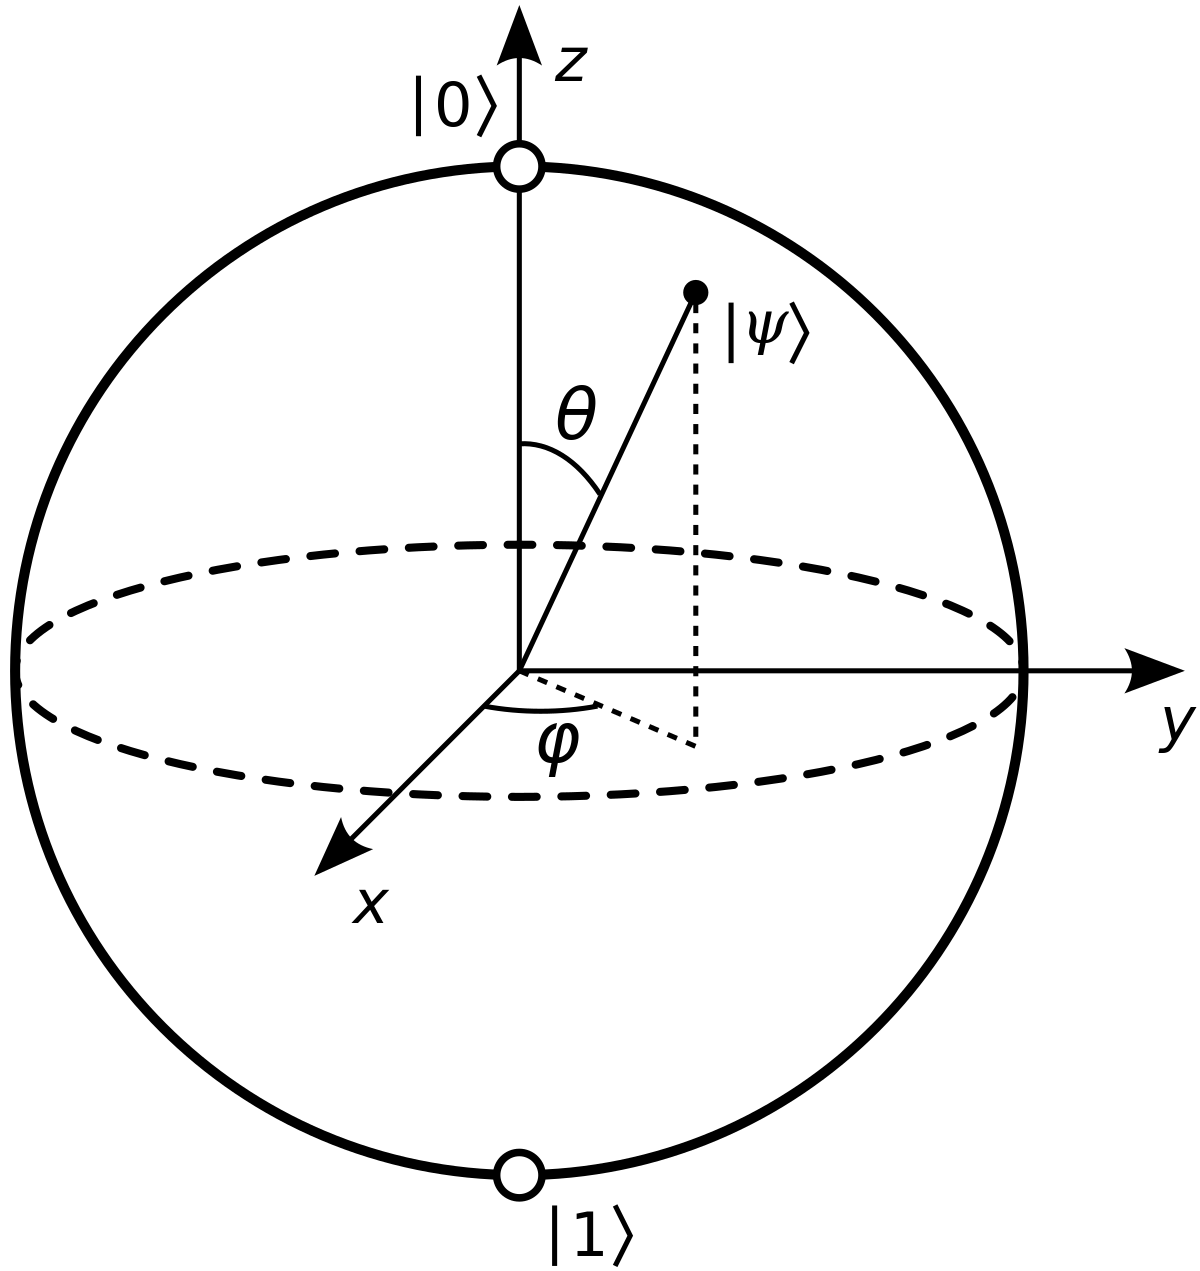
\includegraphics[width=0.3\textwidth]{figures/bloch_sphere.png}
    \caption{Bloch sphere representation of a qubit \cite{wiki:qubit}}
    \label{fig:bloch-sphere}
\end{figure}
While the classical bit only exists in 2 points, the north and south poles, the qubit extends the quantum state to any position on the surface of the cube. \cite{wiki:qubit,book:Nielsen-Chuang-2010}\medbreak

The visual explanation unfortunately fades when we consider multiple qubits: in that case, it is much easier to talk about a $2^n$ dimensional basis. For example, with 2 qubits, 4 basis elements describe a quantum state:

\begin{equation}
    \ket{\phi} = \alpha \ket{00} + \beta \ket{01} + \gamma \ket{10} + \delta \ket{11}
\end{equation}

where $\alpha,\beta,\gamma,\delta \in \mathbb C$ and normalize to 1, and $\ket{\phi} \in \mathbb{C}^4$.\medbreak

\section{Quantum Tomography}\label{section:quantum-tomography}
As described in \ref{introduction:quantum-tomography}, Quantum Tomography studies the reconstruction of a quantum state described by a density matrix $\rho$. It builds upon the Born rule, which states that given a system state $\ket \psi$ and an observable operator $O$, the probability of occurrence of an eigenvalue $m$ of $O$ will be 
\begin{equation}
    p(m) = \braket{\psi | P_m| \psi} = \lvert\braket{m|\psi}\rvert^2
\end{equation}
where $P_m = \ket m \bra m$ is a projection onto the eigenstate of $O$ with eigenvalue $m$ (and corresponding eigenvector $\ket m$). The system is measured using $P_m$ with the outcome being an eigenstate $m$ (to be precise it is measured with the collection $\{P_m\}$ associated to $O$). Note that the term operator will be used interchangeably with the term matrix in what follows, as they are equivalent in this context.\medbreak

In general, one observable is however not enough as it only measures a specific aspect of a state. We will therefore create a collection of observables $\mathcal{O}$ with $O \in \mathcal{O}$, which will allow us to fully describe our state. In the situation when we have access to the entire set $\mathcal{O}$, we talk about a \ti{complete measurement} case. Of course, doing one measurement with an observable is not informative enough, and in order to obtain any statistically significant estimate for the probability of projector, we measure an ensemble $m$ of identically prepared quantum states for each $O$. \medbreak

In the following sections, we will provide a more thorough mathematical background and describe in more detail the different components that constitute Quantum Tomography.
\subsection{Mathematical description} \label{background:Quantum Tomography:math}

\subsubsection*{Pure states, mixed states and density matrix}
A \textit{pure state} is a quantum state that can be represented using a finite or infinite complex vector $\ket \psi$, element of a Hilbert space, and of norm 1. Equivalently, it is a state that can not be expressed as a convex combination of other quantum states \cite{wiki:density-matrix}.\medbreak

A \textit{mixed state} $\ket \phi$, on the other hand, is a probabilistic mixture of pure states $\ket {\psi_j}$. Mixed states usually arise in situations when we do not know from which states our system state is constituted. This means that we can not anymore represent our system state as a vector, and must resort to a more general form: the density matrix.\medbreak

A \textit{density matrix} $\rho \in \mathbb{C}^{d \times d}$, with $d = 2^n$ and $n$ the number of qubits, is a matrix that represents a general quantum state. It is written as
\begin{equation}
    \rho = \sum_{j} p_j \ket{\psi_j} \bra{\psi_j}
\end{equation}
where $p_j$ is the probability of $\ket{\psi_j}$.\medbreak

By construction, we can see that the properties of a density matrix are that it is Hermitian ($\rho = \rho^{\dagger}$), positive semi-definite ($\rho > 0$), and satisfying $\tr(\rho) = 1$. The rank of this matrix also allows us to easily distinguish between a pure state of rank 1, and a mixed state of any rank between 2 and $2^n$, where $n$ is the number of qubits.

\subsubsection*{Born rule, observable and POVM}

The Born rule is a fundamental postulate in Quantum Mechanics that connects the wave function to its measurement. It states that ``the probability density of finding a system in a given state, when measured, is proportional to the square of the amplitude of the system's wavefunction at that state" \cite{wiki:born-rule}.\medbreak

It is described by a collection of orthogonal projective measurements $\{P_m\}$ with $P_mP_{m'}=\delta_{mm'}P_m$. This collection relates to an \textit{observable}, represented by a Hermitian matrix $O$. This property allows it to have a spectral decomposition
\begin{equation}
    O = \sum_m m P_m
\end{equation}
where $P_m$ is the projection onto the eigenspace of $O$ associated to eigenvalue $m$. An observable corresponds to a physical property that can be measured, for example, the position, momentum or spin of a particle.\medbreak

In the case where our state $\ket \psi$ is pure, the Born rule is formulated as
\begin{equation}
    p(m) = \braket{\psi|P_m|\psi}
\end{equation}
and can be further generalized to a mixed state, represented with a density matrix $\rho$
\begin{equation}\label{eq:quantum-measurement}
    p(m) = \tr(\rho P_m)
\end{equation}

A small example of such a collection are the projectors operators of the \textit{computational basis} ($\ket 0$ and $\ket 1$). The resulting matrices are $P_0 = \ket 0 \bra 0$ and $P_1 = \ket 1 \bra 1$. If we have that $\ket \psi = a \ket 0 + b \ket 1$, then $p(0) = \braket{\psi|P_0^\dagger P_0|\psi} = \braket{\psi|P_0|\psi} = |a|^2$ (by idempotency of a projector matrix).\medbreak
    
In the context of Quantum Tomography, the most relevant aspect to measure is the spin: in each direction $\{x,y,z\}$, we use a Pauli matrix to probe whether a qubit is spin up or down \cite{book:Nielsen-Chuang-2010,wiki:born-rule}. \medbreak

Note that, while projective measurements are the most common measurement operator, they are a specific case of the \textit{Positive Operator-Valued Measure} (POVM). This generalized measure does not enforce the orthogonality property and only requires the collection $\{F_m\}$ to be Hermitian, positive semi-definite operators on a Hilbert space, and satisfy the completeness relation
\begin{equation}
    \sum_m F_m = I
\end{equation}


\subsection{Data generation}
There are multiple ways through which one can obtain data for quantum tomography: using a real-world dataset is a possibility, however for that, you need access (or need to know someone who has) to a quantum computer. An easier approach is simply to simulate the data. It has its downsides, notably the fact that it may not be representative of true data. In our experiments, however, we will stick to synthetic data as it is very flexible and better suited for algorithm research and numerical experiments, due to the low iteration time.\medbreak

When using synthetic data generation, 2 main options are usually considered: separate qubit or mixed qubit.


\subsubsection*{Separate qubit data generation}\label{section:sep-qub-dg}
Separate qubit data generation (also called the ``Pauli basis measurements" in \cite{Guta20}) is a process through which we can find the probability associated with an outcome $\mb s = (s_1, s_2 \dots, s_n) \in \mathcal{R}^n := \{-1, 1\}^n $ for an observable $\mb a = (a_1, a_2 \dots, a_n) \in \mathcal{E}^n := \{x,y,z\}^n$ (we adopt the same notations as in \cite{MA17} here and make them more specific than in the introduction \ref{section:litterature-review}).\medbreak

The observable $\sigma_{a_i}$ for a qubit can be in $\{\sigma_x, \sigma_y, \sigma_z\}$, where $\sigma_i \in \mathbb{C}^{2 \times 2}$ is one of the Pauli matrices. These matrices are written as follows:
\begin{equation}
    \sigma_x  = \begin{pmatrix}
        0 & 1\\
        1 & 0
    \end{pmatrix}\quad
    \sigma_y = \begin{pmatrix}
        0 & -i\\
        i & 0
    \end{pmatrix}\quad
    \sigma_z = \begin{pmatrix}
        1 & 0\\
        0 & -1
    \end{pmatrix}
\end{equation}
They distinguish themselves by being Hermitian, unitary, and having eigenvalues $\{-1, 1\}$. They correspond to measuring the projection of the spin on the qubit, an intrinsic property of a particle analogous to angular momentum, along a particular dimension \cite{wiki:pauli-matrices}.
We thus have a total of $3^n$ possible experimental observables and $2^n$ possible outcomes for each observable. Based on the observable and outcome, we can create the operator $P^\mb a_{\mb s} = P^{a_1}_{s_1} \otimes \dots \otimes P^{a_n}_{s_n}$, which corresponds to the projector for this $(\mb a,\mb s)$ pair. The term $P^{a_i}_{s_i}$ corresponds to the orthogonal projection associated to the eigenvalue $s_i$ in the diagonalization of $\sigma_{a_i}$, which in turn can be rewritten as $\sigma_{a_i} = -1P^{a_i}_{-1} + 1P^{a_i}_1$ due to its Hermitian property. Note that under this notation, $\mb a$ and $\mb s$ are both vectors \ti{and} indices. Reminding ourselves of the POVM and Born's rule we saw in \ref{background:Quantum Tomography:math}, we can formulate the main equation as


\begin{equation}
    \forall \mb s \in \mathcal{R}^n, p_{\mb a,\mb s} = \Pr(R^{\mb a} = \mb s) = \tr(\rho P^{\mb a}_{\mb s})
\end{equation}
where $R^\mb{a} \in \mathcal{R}^n$ is the random vector outcome of the measurement with $\mb a$ and $p_{\mb a,\mb s}$ the probability linked to that pair. We can see that we recover the projective measurement (or more generally the POVM), only extended to the multi-qubit case by the Kronecker product applied to the projectors $P^{\mb a}_\mb{ s}$.\medbreak

An important element to take into account when working with this method in practice is that, while it is the theoretically correct approach, it requires on the order of $6^n = 2^n 3^n$ operations, making it costly.

% Note that there is a slight confusion between the term observable for a qubit (i.e. a Pauli matrix) and an observable to measure the system (in this case the Kronecker product of projection matrices).


\subsubsection*{Mixed qubit data generation}\label{section:mixed-qub-dg}

Mixed qubit data generation (also called ``Pauli observables" in \cite{Guta20}) is an alternative approach, where instead of calculating the probability for each observable/outcome pair, we will directly approximate the expected value linked to this observable. Its calculation is much more straightforward: if we call $A_m$ the observable of which we calculate the expected value, then $A_m = \sigma_{m_1} \otimes \sigma_{m_2} \dots \otimes \sigma_{m_n}$ with $n$ the number of qubits and $m_i$ identifying the Pauli matrix for qubit $i$ for combination $m$ (the notation is the same as in \cite{meth:bayesian:Langevin:ACMT2024}). The measured value for each observable is $\hat p_m \in[-1, 1]$. This results in a total of $4^n$ combinations ($\sigma_{m_i} \in \{I, \sigma_x, \sigma_y, \sigma_z\}$), hence less costly than the separate qubit process.

%\section{Pointwise estimation methods}
\newpage

\section{Markov Chain Monte Carlo methods}\label{section:mcmc-methods}
Markov Chain Monte Carlo (MCMC) methods are a class of sampling algorithms. Sampling from a probability distribution is relevant when we want to compute some statistic about it, for example, the mean. In most cases, the target distribution $\pi(\mb x)$ has high dimensionality as we work in the space of parameters of statistical models. MCMC is particularly important in the context of \ti{Bayesian inference}. In this case, $\pi(\mb x)$ corresponds to the posterior distribution from which we want to sample, and whose probability density function usually corresponds to a complex expression. \medbreak

Various methods exist for sampling from simple distributions, the most famous being the inverse transform method, rejection sampling, or importance sampling. All these methods however have drawbacks: inverse transform requires an analytical solution for the cumulative density function, which is usually not possible to obtain for complex probability density functions as it requires a proper integral; rejection sampling and importance sampling do not have this problem, but they suffer from the curse of dimensionality - once your dimension grows, the sampling becomes very inefficient. MCMC methods solve these issues, with certain methods being more suitable than others depending on the specific situation.\medbreak

We will now cover several aspects that make up MCMC: Bayesian inference in \ref{section:background:mcmc:bayesian-inference}, the theoretical guarantees behind the MCMC methods in \ref{section:background:mcmc:theory}, and finally the 3 main algorithms we will be concerned about in this thesis, Metropolis-Hastings in \ref{section:Metropolis-Hastings}, Gibbs sampling in \ref{section:gibbs} and Langevin sampling in \ref{section:ula}.

\subsection{Bayesian inference}\label{section:background:mcmc:bayesian-inference}
As its name suggests, Bayesian inference relies on Bayes theorem. In the context of algorithms, it states that given data $\mb{D}$ and parameters $\boldsymbol{\theta}$, the \textit{posterior} distribution $\pi(\btheta|\mb{D})$ is calculated as 
\begin{equation} \label{eq:posterior-with-marginal}
    \pi(\boldsymbol{\theta}|\mb{D}) = \frac{\pi(\mb{D}|\boldsymbol{\theta})\pi(\boldsymbol{\theta})}{\pi(\tb D)} = \frac{\pi(\mb{D}|\boldsymbol{\theta})\pi(\boldsymbol{\theta})}{\int_{\boldsymbol{\theta}} \pi(\mb{D}|\boldsymbol{\theta}) \pi(\boldsymbol{\theta})d\boldsymbol{\theta}}
\end{equation}
where $\pi(\mb{D}|\btheta)$ is the \ti{likelihood} of data given the parameters and $\pi(\btheta)$ the \ti{prior} distribution we put on the parameters. The denominator
\begin{equation}
    \pi(\mb{D}) = {\int_{\boldsymbol{\theta}} \pi(\mb{D}|\boldsymbol{\theta}) \pi(\boldsymbol{\theta})d\boldsymbol{\theta}}
\end{equation} 
is called the \ti{marginal}, and corresponds to a normalizing constant. It is in practice intractable to calculate as it involves performing a very high dimensional integral numerically, which is unstable. The good news is that in the context of MCMC methods, the normalizing factor is not important and we can safely remove it. This gives the following posterior:
\begin{equation} \label{eq:posterior-without-marginal}
    \pi(\boldsymbol{\theta}|\mb{D}) \propto {\pi(\mb{D}|\boldsymbol{\theta}) \pi(\boldsymbol{\theta})}
\end{equation}
Getting samples from $\pi(\boldsymbol{\theta}|\mb{D})$ allows us to compute integrals, a technique called Monte Carlo integration. For example, if we have a function $g$ defined on $\mathbb{R}^m$ and we want to approximate its integral on a subset $\Omega \subseteq \mathbb R^m$, we can sample $N$ values uniformly $\{\btheta_i\}_{i=1}^N \in \Omega$ and calculate 
\begin{equation}
    \int_\Omega g(\btheta) d\btheta \approx \frac{1}{N} \sum_{i=1}^{N} g(\btheta_i)
\end{equation}
The law of large numbers ensures that with $N \rightarrow \infty$, the discrete sum converges to the true integral \cite{wiki:monte-carlo-integration}.\medbreak

In statistics, integrals are of particular interest to us as they correspond to expectations. If we have function $f(\boldsymbol{\theta})$ defined on some set $\boldsymbol{\Theta}$, then
\begin{equation}
    \mathbb E_{\boldsymbol \theta \sim \pi(\btheta|\mb{D})}\left[f(\boldsymbol{\theta})\right] = \int_{\boldsymbol{\theta}} f(\boldsymbol{\theta})\pi(\btheta|\mb{D}) d\boldsymbol{\btheta} \approx \frac{1}{N} \sum_{i=1}^{N} f(\boldsymbol{\theta}_i)
\end{equation}
where $\{\boldsymbol{\theta}_i\}^N_{i=1}$ are samples from $\pi(\btheta|\mb{D})$. This allows us to compute estimates for a random variable (with $f(\btheta) = \btheta$), vector, or matrix, the last one being the most relevant in Quantum Tomography. In that case, the parameters correspond to the density matrix $\rho$, and the data to the projectors $P^{\mb a}_{\mb s}$ and the empirical probabilities $\hat p_{\mb a,\mb s}$. By first putting a prior on $\rho$, we can obtain a sample estimate of $\rho$, balanced by the data we have. This is where the term \ti{inference} comes from, as we infer $\rho$ from the data and prior.

\subsection{Theoretical guarantees}\label{section:background:mcmc:theory}
In contrast to Monte Carlo methods where the samples are independent, MCMC builds a \ti{Markov chain} of samples $\mb x^{(1)}, \dots, \mb x^{(R)}$, which are dependent (we use $\mb x$ instead of $\btheta$ to be as general as possible). As a reminder, a sequence $\mb X^{(1)}, \mb X^{(2)} \dots \mb X^{(R)}$ of random variables is a Markov chain if
\begin{equation}
    \Pr(\mb X^{(r+1)} \in A|\mb x^{(1)}, \dots, \mb x^{(r)}) = \Pr(\mb X^{(r+1)}|\mb x^{(r)})
\end{equation}
where $\mb x^{(i)}$ is a realization of $\mb X^{(i)}$ on domain $A$ (which is usually multidimensional hence the bold notation, however in our definitions it will be one-dimensional). One question remains: how can we make sure that samples we obtain from some Markov chain indeed come from the distribution we sample from? To answer this, we need to review several properties of Markov chains.\medbreak

A \ti{transition kernel} $k$ is a function that fully characterizes a Markov chain. It gives the probability of transitioning from one state to another in a chain: in the continuous case, this corresponds to conditional function $k(\mb x^{(r+1)}| \mb x^{(r)})$ and the discrete case, it is a transition matrix $P$. We say that our chain in \ti{invariant} to a distribution $\pi(\mb x)$ if 
\begin{equation}
    \pi(\mb x^*) = \int k(\mb x^*|\mb x) \pi(\mb x)d\mb x
\end{equation}
This corresponds to saying that our chain admits a \ti{stationary} distribution, or equivalently that the \ti{marginal} distributions of $\mb X^{(r)}$ and $\mb X^{(r+1)}$ are the same. The distribution $\pi(\mb x)$, called the \ti{target} density, corresponds to the distribution we want to sample from in the context of MCMC. It is important to note that not all chains admit a stationary distribution, and a few properties must be respected. We will cover the discrete case for brevity reasons, but this of course extends to the continuous one \cite{mcmc:slides:Rigon2024Mar,wiki:markov-chain}.
\begin{itemize}
    \item \tb{Irreducibility}: a Markov chain is \ti{irreducible} if it explores the entire sample space, and does not get stuck in local regions. Formally, if $\mb X^{(r)}\in \mathbb{N}$, this corresponds to the condition 
    \begin{equation}
        \Pr(\tau_j < \infty | \mb x^{(0)} = j') > 0\quad \forall j,j' \in \mathbb{N}
    \end{equation} 
    where $\tau_j = \inf\{r\geq 1: \mb X^{(r)} = j\}$ is the first passage time for which the chain is equal to $j$ (defined as $\infty$ if $\mb X^{(r)} \neq j$ for every $r\geq 1$) and $\Pr(\tau_j < \infty | \mb x^{(0)} = j')$ the probability of return to $j$ in a finite number of steps.
    \item \tb{Aperiodicity}: a Markov chain is \ti{aperiodic} if it does not have any deterministic cycles. Formally, we say that a state $j$ is aperiodic if the set $\{r\geq1: [P^r]_{jj} > 0\}$ has no common divisor other than 1. A chain is aperiodic if all of its states are aperiodic.
    \item \tb{Harris recurrence}:  a Markov chain is \ti{recurrent} if it visits any region of the sample space sufficiently often. Formally, a state $j$ of a discrete irreducible Markov chain is recurrent if and only if
    \begin{equation}
        \Pr(\tau_j < \infty |\mb x^{(0)} = j) = \Pr(\mb X^{(r)} = j \text{ for infinitely many } r | \mb x^{(0)}=j) = 1
    \end{equation}
    In other words, it means that this state is visited infinitely often. If we have all the states that are recurrent, then the chain is called recurrent. If additionally this chain admits an invariant distribution, then it is Harris positive (also called positive recurrent).
    \item \tb{Ergodicity}: a Markov chain in \ti{ergodic} if every state is ergodic. A state $j$ is ergodic if it is aperiodic and positive recurrent. Intuitively, this property means that we can reach every state with a probability greater than 0.
\end{itemize}
We can finally state the main result that allows us to use Markov chains for MCMC \cite{mcmc:RobertCasella2004}:
\begin{boxedthm}
    A Markov chain Monte Carlo (MCMC) method converges to a distribution $\pi(\mb x)$ if the underlying Markov chain is ergodic with an equilibrium distribution $f(\mb x) = \pi (\mb x)$.
\end{boxedthm}

A closely related theorem that provides a guarantee similar to the law of large numbers for Markov chains is the \ti{Ergodic} Theorem \cite{mcmc:slides:Rigon2024Mar}:

\begin{boxedthm}
    Let the Markov chain $(\mb X^{(r)})_{r\geq 1}$ be Harris positive with stationary distribution $\pi$, and $g$ be integrable with respect to $\pi$. Then,
    \begin{equation}
        \frac{1}{R}\sum_{r=1}^{R}g(\mb X^{(r)}) \rightarrow \int g(\mb x) \pi(\mb x) d \mb x \quad \text{when } R \rightarrow \infty
    \end{equation} 
    almost surely.
\end{boxedthm}

\subsection{Metropolis-Hastings algorithm}\label{section:Metropolis-Hastings}
The \ti{Metropolis-Hastings} algorithm is the most well-known and used MCMC algorithm. The Markov chain of samples is built by doing a random walk, with an acceptance/rejection step. It works as follows: given that we are currently located at $\mb x \in \mathbb{R}^n$, we will sample a potential candidate $\mb x^*$ from $q(\mb x^*|\mb x)$ where $q$ is called the \ti{proposal} (or \ti{jumping}) distribution. This $q$ is analogous to the kernel we saw in \ref{section:background:mcmc:theory}, although not exactly as we will see later (see equation \ref{eq:mh-transition-kernel}). Next, we will compute the \ti{acceptance} probability of this sample:

\begin{equation}
    \alpha(\mb x^*, \mb x) = \min\left(1, \frac{\pi(\mb x^*) q(\mb x|\mb x^*)}{\pi(\mb x) q(\mb x^*|\mb x)}\right)
\end{equation}
where $\pi(\mb x)$ is the posterior distribution we would like to sample from. Note that we can simplify this criterion in case the proposal density is symmetric ($q(\mb x^*|\mb x) = q(\mb x|\mb x^*)$):
\begin{equation}
    \alpha(\mb x^*, \mb x) = \min\left(1, \frac{\pi(\mb x^*)}{\pi(\mb x)}\right)
\end{equation}
This happens often in practice, as the Gaussian distribution is a common choice of proposal.
A second comment is that, as mentioned in section \ref{section:background:mcmc:bayesian-inference}, the normalizing constant of the posterior is not important: it gets simplified in the numerator and denominator as it does not depend on $\mb x$, nor $\mb x^*$ (only the data \tb D, see equation \ref{eq:posterior-with-marginal}). \medbreak

After this computation, we will accept $\mb x^*$ with probability $\alpha$. In practice, this involves, for example, sampling a value $u \sim U(0,1)$, and accepting if $ u \leq \alpha$. This procedure is repeated until the desired number of samples is obtained, with some part of samples that we discard at the beginning. This period is called the \ti{burn-in} period and corresponds to the duration when the samples we obtain are not part of the equilibrium distribution.
We usually talk about \textit{convergence} when the samples come from $\pi$ (the posterior distribution we want to sample from), or that the Markov chain has \textit{mixed}. A pseudocode for the algorithm could be:\medbreak

\begin{algorithm}[H]
    \DontPrintSemicolon
    \SetKwInOut{Input}{Input}
    \SetKwInOut{Output}{Output}

    %\underline{Prob-estimator}\;
    \Input{$\mb x^{(0)} \in \mathbb{R}^n, T \in \mathbb{N}$}
    \Output{$\mb x^{({1})} \in \mathbb{R}^n, \mb x^{(2)}, \dots, \mb x^{(T)}$}
    \For{$t\gets 1:T$}{ 
        Sample $\mb x^* \sim q(\mb x|\mb x^{(t-1)})$\;
        $\alpha = \min\left(1, \frac{\pi(\mb x^*) q(\mb x^{(t-1)}|\mb x^*)}{\pi(\mb x^{(t-1)}) q(\mb x^*|\mb x^{(t-1)})}\right)$\;
        Sample $\mb x^* \sim U(-0.5, 0.5)$\;
        \eIf{$u \leq \alpha$}{
            \tcp*[l]{Accept $\mb x^*$}
            $\mb x^{(t)} \gets \mb x^*$
        }{
            \tcp*[l]{Reject $\mb x^*$}
            $\mb x^{(t)} \gets \mb x^{(t-1)}$
        }
    }
    \caption{Metropolis-Hastings algorithm}
\end{algorithm}\medbreak
where $T$ is the number of iterations.\medbreak

Note that in most implementations, it is common practice to use $\log(\alpha)$ for the calculation of the acceptance probability, instead of $\alpha$ directly. This allows to avoid numerical problems due to divisions by small numbers and underflow/overflow that might occur when handling double-precision floats. In addition, using the logarithm combines nicely with distributions based on the exponential family, allowing for a $\log(\exp)$ simplification.\medbreak

We have in section \ref{section:background:mcmc:theory} talked about convergence for Markov chains to the posterior distribution, but have not talked how that would work in practice. A very handy way is to use the \ti{detailed balance} condition.

\begin{boxedthm}
    A Markov chain $(\mb X^{(r)})_{r\geq1}$ with transition kernel $k$ satisfies the detailed balance if there exists a function $f$ such that 
    \begin{equation}
        k(\mb x|\mb x^*) f(\mb x) = k(\mb x^*|\mb x) f(\mb x^*)
    \end{equation}
\end{boxedthm}
In this context, we also talk about \ti{reversibility}:

\begin{boxedthm}
    a Markov chain $(\mb X^{(r)})_{r\geq1}$ is \ti{reversible} if
\begin{equation}
    \Pr(\mb X^{(r)} | \mb X^{(r+1)}) = \Pr(\mb X^{(r+1)} | \mb X^{(r)})
\end{equation}
\end{boxedthm}
Finally, we can reach an important and useful result for MCMC:

\begin{boxedthm}
    if a Markov chain $(\mb X^{(r)})_{r\geq1}$ satisfies the detailed balance with $\pi$ a probability density function, then $\pi$ is the stationary density, and chain is reversible.
\end{boxedthm}

This result means that, as long as we satisfy the detailed balance with our MCMC algorithm, we will converge to the posterior distribution $\pi$. In the case of Metropolis-Hastings, the transition kernel is 
\begin{equation}\label{eq:mh-transition-kernel}
    k\left(\boldsymbol{x}^* \mid \boldsymbol{x}\right)=\alpha\left(\boldsymbol{x}^*, \boldsymbol{x}\right) q\left(\boldsymbol{x}^* \mid \boldsymbol{x}\right)+\delta_{\boldsymbol{x}}\left(\boldsymbol{x}^*\right) \int q(\boldsymbol{s} \mid \boldsymbol{x})\{1-\alpha(\boldsymbol{s} \mid \boldsymbol{x})\} \mathrm{d} \boldsymbol{s}
\end{equation}
where $\delta_{\mb x}(\mb x^*)$ is a point mass at $\mb x$. Putting this kernel into the detailed balance condition, one can derive that the equality indeed holds. The only element that we have not discussed so far is the ergodicity condition. Although is depends on $\pi$ and $q$, it is typically true under very mild conditions, which can be checked in, for example, \cite{mcmc:RobertCasella2004}.\medbreak

A final element to take into account with theoretical convergence guarantees is that in real-world experiments, the algorithm may take a very long time to converge, making it impractical for real use. In these situations, one could for example investigate different proposals, change the duration of the burn-in period, or even swap Metropolis-Hastings for another algorithm. Various metrics exist to quantify the convergence, such as the effective sample size or $\hat R$, but also visual checks, which are effective for checking if the chain has mixed. It is also common practice to run several chains from different starting points and assess the overall performance. More details about practical considerations can be found in \cite{mcmc:gelman2013bayesian}.

\subsection{Gibbs sampling algorithm}\label{section:gibbs}
The Gibbs sampling algorithm takes a different approach compared to Metropolis-Hastings in that it splits the joint distribution $\pi(\mb x) = \pi(x_1, x_2, \dots, x_n)$ with $\mb x \in \mathbb{R}^n$ into one-dimensional conditionals, and then step samples from each conditional $\pi(x_i|\mb x_{-i}) = \pi(x_i|x_1,\dots,  x_{i-1}, x_{i+1}, \dots, x_n)$ iteratively. It can also be generalized to blocks, where instead of sampling from a one-dimensional distribution, we sample from a joint conditional. \medbreak

It is, in its simplest form, an \ti{unadjusted} algorithm, as it does not involve an accept/reject step.
A pseudocode for it can be the following:\medbreak

\begin{algorithm}[H]
    \DontPrintSemicolon
    \SetKwInOut{Input}{Input}
    \SetKwInOut{Output}{Output}

    \Input{$\mb x^{(0)}, T \in \mathbb N$}
    \Output{$\mb x^{(1)}, \mb x^{(2)}, \dots, \mb x^{(T)}$}
    \For{$t\gets 1:T$}{ 
        $\mb x^{(t)} \gets \mb x^{(t-1)}$\;
        \For{$i\gets 1:n$}{
            \tcp*[l]{Sample from the conditional and set $i$-th element to this value}
            $\mb x_{i}^{(t)} \sim \pi(x_i|\mb x_{-i}^{(t)})$\;
        }
    }
    \caption{Gibbs algorithm}
\end{algorithm}
Note that the inner loop updates the current $\mb x^{(t)}$, and not a copy. This implies that at iteration $i$, we are using the conditioned value set at $i-1$ for $x^{(t)}_{i-1}$, and not the one set at $x^{(t-1)}_{i-1}$.\medbreak

The main advantages of Gibbs sampling is that we do not need to tune the proposal distributions, as well as the fact that all samples are accepted. The downside of course is that we need to be able to derive and sample from the conditional, especially doing so efficiently as otherwise this approach becomes very costly. A more general algorithm called \textit{Metropolis-within-Gibbs}, involves sampling from the conditional using Metropolis-Hastings, and in that case this may involve an accept/reject step (an example of which is the prob-estimator in section \ref{section:prob-estimator} or the MHGS algorithm in section \ref{section:mhs-and-mhgs}). \medbreak

In the case of standard Gibbs, we may view the conditionals we sample from as proposal distributions $q(\mb x^*|\mb x)$. This in turn shows us why this algorithm is unadjusted, as the acceptance probability $\alpha$ is always equal to 1 \cite{mcmc:slides:Rigon2024Mar}. If we call $\mb x^* = (x_1^{(t)}, \dots, x_{i}^*, \dots, x^{(t)}_{n})$ and $\mb x = (x_1^{(t)}, \dots, x_{i}^{(t)}, \dots, x^{(t)}_{n})$, then

\begin{equation}
    \alpha(\mb x^*|\mb x) = \frac{\pi(\mb x^*) q(\mb x|\mb x^*)}{\pi(\mb x) q(\mb x^* |\mb x)} = \frac{\pi(x_i^*|\mb x_{-i}^*)\pi(\mb x^*_{-i}) \pi(x_i|\mb x^*_{-i})}{\pi(x_i|\mb x_{-i})\pi(\mb x_{-i}) \pi(x_i^*|\mb x_{-i})} = \frac{\pi( x_i^*|\mb x_{-i})\pi(\mb x_{-i}) \pi(x_i|\mb x_{-i})}{\pi(x_i|\mb x_{-i})\pi(\mb x_{-i}) \pi(x_i^*|\mb x_{-i})} = 1
\end{equation}
where we have used the fact that $\mb x^*_{-i} = \mb x_{-i}$.


\subsection{Unadjusted Langevin algorithm}\label{section:ula}
One big downside with Metropolis-Hastings or Gibbs sampling is that they can take a long time to converge, especially in a very high-dimensional setting. The Unadjusted Langevin algorithm (ULA) tackles this problem by using the gradient information of the posterior. The downside, of course, is that we must be able to calculate it, but in the case we can, it can drastically speed up the convergence.\medbreak

The algorithm draws its name from \ti{Langevin diffusion} (also called \ti{Îto diffusion}), a stochastic differential equation (SDE), written as follows:
\begin{equation}
    \mathrm{d}\mb X_t = -\nabla V(\mb x)\mathrm{d}t + \sqrt{2}\mathrm{d}\mb B_t
\end{equation}
where $\mb X_t$ is the position of a particle in a potential $V(\mb x)$ and $\mb B_t$ is the time derivative of the standard Brownian motion. A SDE is a differential equation where one or more of the terms is a stochastic process and results in a solution which is also a stochastic process. In the case of Langevin diffusion, the solution happens to be a stationary process $p_{\infty}(\mb x) \propto \exp(-V(\mb x))$, which is very handy in the context of MCMC. If we set $V(\mb x) = -\log(\pi(\mb x))$, then we can simulate the SDE and obtain samples from $p_\infty = \pi$:
\begin{equation}    
    \mathrm{d}\mb X_t = \nabla \log(\pi(\mb x))\mathrm{d}t + \sqrt{2}\mathrm{d}\mb B_t
\end{equation}

Of course, to simulate, we must discretize the SDE in some way, and in this case \textit{Euler-Maruyama approximation} is what is commonly used. This results in
\begin{equation}
    \mb X^{(k+1)} - \mb X^{(k)} = \tau \nabla \log\pi(\mb X^{(k)}) + \sqrt{2\tau}(\mb B^{(k+1)} - \mb B^{(k)})
\end{equation}
where $\tau$ is a step size that can be changed over time and $(\mb B^{(k+1)} - \mb B^{(k)}) \sim N(\mb 0, \mb I)$. We can then rewrite it as follows:
\begin{equation}
    \mb X^{(k+1)} = \mb X^{(k)} + \tau \nabla \log\pi(\mb X^{(k)}) + \sqrt{2\tau}\boldsymbol{\xi}^{(k)}
\end{equation}
where $\boldsymbol{\xi}^{(k)} \sim N(\mb 0, \mb I)$. Note that the true solution can be computed with $\mb X(k\tau)$. The pseudocode can be written as follows:\medbreak
\begin{algorithm}[H]
    \DontPrintSemicolon
    \SetKwInOut{Input}{Input}
    \SetKwInOut{Output}{Output}

    \Input{$\mb x^{(0)}, K, \tau^{(1)}, \dots, \tau^{(K)}$}
    \Output{$\mb x^{(1)}, \mb x^{(2)}, \dots, \mb x^{(K)}$}
    \For{$k\gets 1:K$}{ 
        $\boldsymbol{\xi}^{(k)} \sim N(\mb 0, \mb I)$\;
        $\mb x^{(k+1)} = \mb x^{(k)} + \tau^{(k)} \nabla \log\pi(\mb x^{(k)}) + \sqrt{2\tau^{(k)}}\boldsymbol{\xi}^{(k)}$\;
    }
    \caption{Unadjusted Langevin algorithm}
\end{algorithm}
with $K$ the number of iterations and $\tau^{(k)}$ the step size.  \medbreak

ULA can be seen as noisy gradient ascent, which is why it performs better than Metropolis-Hastings or Gibbs. By utilizing the gradient information, we are able to sample more often the regions of high density. The cost of computing the gradient is usually compensated by faster convergence times, making it often an algorithm of choice if the gradient of the posterior can be computed. The algorithm is relevant in this thesis due to its use in the Projected Langevin method (see section \ref{section:projected-langevin}). Note that there also exists a method called \textit{Metropolis-adjusted Langevin algorithm} (MALA), which generalizes this approach with an accept/reject step, but we will not go into the details here \cite{mcmc:langenvin-blog:Ansari2024Apr, wiki:MALA}.

\chapter{Overview of relevant methods} \label{section:relevant-methods}
In this chapter, we will introduce two MCMC algorithms that are in relevant in the context of this thesis: the \ti{prob-estimator} (in \ref{section:prob-estimator}) and the \ti{Projected Langevin algorithm} (in \ref{section:projected-langevin}). They will be useful in Chapter \ref{section:numerical-exp} where we will be comparing them in numerical experiments and Chapter \ref{section:algo-vs-prior} where we will be presenting 2 new algorithms derived from them.\medbreak

Note that both papers provide theoretical convergence bounds for the method they propose, however, we will not describe them here as they are not relevant in the context of our experiments. Also note that the notations we use in this chapter differ from the ones used in the MCMC chapter \ref{section:mcmc-methods}, as we prefer to stick to the notations used in the original papers.

\section{Prob-estimator}\label{section:prob-estimator}
Introduced in \cite{MA17}, the \textit{prob-estimator} is a Metropolis-Hastings-based algorithm (more details about it can be found in section \ref{section:Metropolis-Hastings}), where the approximation of the density matrix $\rho$ is done using a sum of rank 1 matrices and sparse coefficients, leading to a rank 1 approximation. The exact solution is written as follows:
\begin{equation}\label{eq:rank1-approx}
    \rho = \sum_{i=1}^d \gamma_i V_i V_i^\dagger
\end{equation}
where $V_i \in \mathbb{C}^{d\times 1}$ are normalized vectors and $\gamma_i \in \mathbb{C}$ are the sparse coefficients with $\sum_{i=1}^d \gamma_i = 1$.\medbreak

We can check that the properties of a density matrix are respected: it is a sum of Hermitian matrices, which also makes $\rho$ Hermitian and positive semi-definite and 
\begin{equation}
    \tr(\rho) = \sum_{i=1}^{d} \gamma_i \tr(V_i V_i^\dagger) = 1
\end{equation}
as $\tr(V_i V_i^\dagger) = 1$ due to the normalization.\medbreak
% \begin{equation}
% \hat \rho = \frac{1}{T}\sum_{t=1}^{(t)}  \left(
% \sum_{i=1}^d \gamma_i^{(t)} V_i^{(t)} (V_i^{{(t)}})^\dagger 
% \right)
% \end{equation}

This way of calculating $\rho$ is analogous to taking an eigenvector decomposition
\begin{equation}
    \rho = U\Lambda U^\dagger
\end{equation}
where $U = (U_1|\dots|U_d)$ with $U_i$ orthogonal to each other and of norm 1, and $\Lambda = \text{diag}(\lambda_1, \lambda_2, \dots, \lambda_d)$ with $\sum_{i=1}^d \lambda_i = 1$ (due to $\rho$ being a density matrix).\medbreak

The advantage of the approach from equation \ref{eq:rank1-approx} is that it does not require the $V_i$ to be orthonormal (as they are in the case of a decomposition of a symmetric/Hermitian matrix). In some sense, the parameter $\gamma_i$ can be thought of as an eigenvalue and $V_i$ its associated eigenvector, even though this is not exactly true as the collection $\{V_i\}$ is not orthogonal. \medbreak

As we are using an MCMC method, we need to formulate the posterior $\pi(\nu | \tb D)$ from which we will be sampling, with $\nu = \sum_{i=1}^d \gamma_i V_i V_i^\dagger$ our parameter matrix and the data $\mb D$ comprised of the projectors $P^{\mb a}_{\mb s}$ and empirical probabilities $\hat p_{\mb a,\mb s}$. In the case of the prob-estimator, the authors use a pseudo-likelihood written as follows
\begin{equation}
    \pi(\tb D| \nu) = \mathcal{L}(\nu, \mb D) = \exp(-\lambda \ell(\nu,\mb D))
\end{equation}
where $\lambda$ is a weight parameter for the likelihood and $\ell(\nu, \mb D)$ the loss function
\begin{equation}
    \ell(\nu, \mb D) = \sum_{\mb a \in \mathcal{E}^n} \sum_{\mb s \in \mathcal{R}^n} \left[\tr(\nu P^{\mb a}_{\mb s}) - \hat p_{\mb a,\mb s}\right]^2
\end{equation}\medbreak
They use separate qubit data generation, thus all details regarding notation can be checked in \ref{section:sep-qub-dg}.
The prior $\pi(\nu) = \pi_1(V_1, \dots, V_d) \pi_2(\gamma_1, \dots, \gamma_d)$ is defined in 2 parts:
\begin{itemize}
    \item For $\pi_1(V_1, \dots, V_d)$, the set $V_1, \dots, V_d$ is i.i.d uniformly distributed on the unit sphere. In practice, this involves first sampling from a standard normal multivariate $\tilde V_i \sim N(\mb 0, \mb I)$, and then normalizing it $V_i = \tilde V_i/||\tilde V_i||$.
    \item For $\pi_2(\gamma_1, \dots, \gamma_d)$, the set $\gamma_1,\dots,\gamma_d$ is sampled from a Dirichlet distribution $\mathcal{D}ir(\alpha_1,\dots,\alpha_d)$ with parameter $\alpha_i > 0$. In order to promote sparsity among $\gamma_1, \dots, \gamma_d$ and get a rank-1 approximation of $\rho$, the parameters are all chosen to be the same, small value: $\alpha_1,\dots,\alpha_d = \alpha = 1/d$. This results in a typical drawing of one $\gamma_i$ close to 1, while others close to 0. In practice, the authors do not sample the Dirichlet distribution directly, and instead use an equivalent formulation: $\gamma_i = Y_i/(\sum_{j=1}^{d} Y_j)$ where $Y_i$ is sampled from a Gamma distribution $Y_i \sim Gamma(\alpha, 1)$.   
\end{itemize}
The posterior is then written as 
\begin{equation}
    \pi(\nu|\tb D) \propto \exp(-\lambda\ell(\nu, \mb D)) \pi(\nu)
\end{equation}
and estimated with 
\begin{equation}
    \hat \rho_{\text{prob}} = \int \nu \pi(\nu|\tb D) d\nu
\end{equation}

As specified above, the prior is split into 2 parts. This is due to the way the algorithm is structured: inside the main loop of Metropolis-Hastings (which goes over iterations $1\rightarrow T$), we also iterate over each dimension $1\rightarrow d$, first for $\gamma$, and then for $V$. This can be seen as doing Metropolis-within-Gibbs. \medbreak

The pseudocode for the algorithm is available below:\medbreak

\begin{algorithm}[H]\label{code:prob}
    \DontPrintSemicolon
    \SetKwInOut{Input}{Input}
    \SetKwInOut{Output}{Output}

    %\underline{Prob-estimator}\;
    \Input{$d = 2^n, \lambda \in \mathbb{R}, \alpha \in \mathbb{R}, T \in \mathbb{N}, V^{(0)} \in \mathbb{C}^{d \times d}, Y^{(0)} \in \mathbb{C}^{d\times 1}$}
    \Output{$\hat \rho \in \mathbb{C}^{d\times d}$}
    $\hat \rho \gets \mb 0$\;
    $\gamma^{(0)} \in \mathbb{R}^{d\times1} \gets Y^{(0)} /(\sum_{i=1}^d Y_i^{(0)})$\;
    \For{$t\gets 1:T$}{ 
    $Y^{(t)} \gets Y^{(t-1)}$\;
    \tcp*[l]{Update $\gamma$}
            \For{$i\gets 1:d$}{
            $\tilde Y \gets Y^{(t)}$\;
            Sample $y \sim U(-0.5, 0.5)$\;
            $\tilde Y_i \gets Y_i^{(t)} \exp (y)$ \;
            $\tilde \gamma \gets \tilde Y /(\sum_{j=1}^d \tilde Y_j)$\;
            $Y_i^{(t)} \gets \begin{cases}
                \tilde Y_i \hspace{0.96cm} \text{with probability} \min\{R(\tilde Y, Y^{(t)}, \tilde \gamma, \gamma^{(t)}, V^{(t-1)}, \lambda, \alpha), 1\} \tcp*[l]{$R$ defined below}\\
                Y_i^{(t)} \hspace{0.63cm}\text{otherwise}
            \end{cases}$
            $\gamma^{(t)} \gets Y^{(t)} /(\sum_{k=1}^d Y_k^{(t)})$ \tcp*[l]{Update all components}
            }
            \;
            $V^{(t)} \gets V^{(t-1)}$\;
            \tcp*[l]{Update $V$}
            
            \For{$i\gets 1:d$}{
            $\tilde V \gets V^{(t)}$\;
            Sample $V \sim N(\mathbf{0}, \mathbf{I})$\;
      
            $\tilde V_i \gets (V + V_i^{(t)})/||V + V_i^{(t)}||_2$\tcp*[l]{Sample from the unit sphere}
            
            $V_i^{(t)} \gets \begin{cases}
                \tilde V_i \hspace{0.96cm} \text{with probability} \min\{A(\tilde V, V^{(t)}, \gamma^{(t)}, \lambda), 1\} \tcp*[l]{$A$ defined below}\\
                V_i^{(t)} \hspace{0.63cm}\text{otherwise}
            \end{cases}$
        }
        \;
        \tcp*[l]{Compute a running average estimate}
        $\hat \rho \gets \frac{1}{t}\sum_{i=1}^{d} \gamma_i^{(t)} V_i^{(t)} (V_i^{(t)})^\dagger  + (1 - \frac{1}{t})\hat \rho $ 
    }
    \caption{Prob-estimator algorithm}
\end{algorithm}\medbreak
where $\lambda$ is a weight parameter for the likelihood, $\alpha$ a scale parameter for the prior, $T$ the number of iterations and $V^{(0)}, Y^{(0)}$ the initial samples. \medbreak

Here, we have that 
\begin{align}
\log R(\tilde Y, Y^{(t)}, \tilde \gamma, \gamma^{(t)}, V^{(t-1)}, \lambda, \alpha) &= - \lambda \ell^{}(\sum_{i=1}^{d} \tilde \gamma_i V_i^{(t-1)} (V_i^{(t-1)})^\dagger, \mb D) + \lambda \ell^{}(\sum_{i=1}^{d} \gamma_i^{(t)} V_i^{(t-1)} (V_i^{(t-1)})^\dagger, \mb D) \\
&\quad + (\alpha - 1) \log\left(\frac{\tilde Y_i}{Y_i^{(t)}}\right) - \tilde Y_i + Y_i^{(t)}
\end{align}

and 
\begin{equation}
\log A(\tilde V, V^{(t)}, \gamma^{(t)}, \lambda) = -\lambda \ell(\sum_{i=1}^{d} \gamma_i^{(t)} \tilde V_i \tilde V_i^\dagger, \mb D) + \lambda \ell^{}(\sum_{i=1}^{d} \gamma_i^{(t)} V_i^{(t)} (V_i^{(t)})^\dagger, \mb D) 
\end{equation}
The curious reader can find the detailed derivations in the appendix \ref{section:appendix:acc-rate-prob}.\medbreak


 Note that there is an element which is ambiguous in the prob-estimator. The lines 7 and 8 of pseudocode \ref{code:prob} correspond to the sampling from $Gamma(\alpha, 1)$. It is however unclear on why this would correspond to obtaining $\tilde Y_i \sim Gamma(\alpha, 1)$. There exists a classical procedure where one uses the inverse transform method and the fact that if $X_i \sim \exp(\lambda)$, then 
\begin{equation}
    \sum_{i=1}^{t} X_i \sim Gamma(t,\lambda)
\end{equation}
however this only works in the case where $t \in \mathbb{N}$. The Wikipedia page \cite{wiki:gamma-dist} mentions that the case with $0 < \alpha < 1$ (assumed with $\beta=1$) is the most challenging to sample from, with new research \cite{mcmc:gamma-sampling:liu2015simulating} still being done on this topic. The Python library \texttt{numpy} does it using a form of rejection sampling\footnote{\texttt{\url{https://github.com/numpy/numpy/blob/main/numpy/random/src/distributions/distributions.c\#220}}}, similar to \cite{mcmc:gamma-sampling:liu2015simulating}. These approaches are however very different from what is done in the prob-estimator, and as the authors do not indicate why it is correct, it is difficult to understand the reasoning behind it.

\newpage
\section{Projected Langevin}\label{section:projected-langevin}

Introduced in the \cite{meth:bayesian:Langevin:ACMT2024} paper (unpublished at the moment of submission of this thesis), the Projected Langevin algorithm is based on an Unadjusted Langevin algorithm (ULA) (more details about it can be found in section \ref{section:ula}). The authors utilize the Burer-Monteiro factorization (introduced in \cite{proj-langevin:Burer2003}) $\rho = Y Y^\dagger$ with $Y \in \mathbb{C}^{d \times r}$ (with $d=2^n$ and $n$ the number of qubits), which corresponds to a low rank (of rank $r$) factorization of $\rho$. This corresponds to considering that the density matrix has a maximum rank of $r$. This also allows us to reduce the dimension of the parameter space from $2d^2$ to $2dr$ by running the MCMC method directly on the $Y$ space. It is important to note that the physical constraints of the problem are still respected, as we assume the matrix $Y$ to belong to the complex hypersphere $C \mathbb{S}^{d\times r} = \{ Y \in \mathbb{C}^{d\times r}: ||Y||_F = 1\}$, leading to a unit trace. The Hermitian and positive semi-definite properties of the density matrix are obtained by construction.\medbreak

In addition to the factorization, the paper proposes a new prior, called the spectral scaled Student-t distribution defined as
\begin{equation}    
\nu_{\theta} (Y) = C_\theta \det(\theta^2I_d + YY^\dagger)^{-(2d+r+2)/2}
\end{equation}
where $\theta$ is a scaling parameter.\medbreak

This prior is an extension of a prior proposed by \cite{Dal20} to the complex domain, where the student-t distribution is a generalization of the Gaussian distribution, allowing for fatter tails. This feature is what promotes sparsity in the eigenvalues of $Y$, favoring a low rank (most samples are close to 0, but occasionally some are large).\medbreak
The used likelihood is similar to the prob-estimator, and is written as 
\begin{equation}
L(Y, \mb D) = \sum^{M}_{i=1} (\hat p_m - \tr(A_mYY^\dagger))^2
\end{equation}
with $A_m$ the Hermitian matrix characterizing the $m^{th}$ experiment and $\hat p_m \in [-1, 1]$ a measured value, whcih together correspond to the data $\mb D$. The authors use mixed qubit data generation, for which more details can be found in section \ref{section:mixed-qub-dg}. \medbreak
Combining these terms, we can obtain a posterior $\hat \nu_{\lambda, \theta}(Y, \mb D) = \exp(-f_{\lambda, \theta}(Y, \mb D))$ with
\begin{equation}
    f_{\lambda, \theta}(Y, \mb D) = \lambda \sum^{M}_{i=1} (\hat p_m - \tr(A_mYY^\dagger))^2 + \cfrac{2d + r + 2}{2}\log \det(\theta^2I_d + YY^\dagger)
\end{equation}
The exponential in this case is useful to us because it allows us to simplify the calculations. ULA requires us to set the potential $V(\mb x) = -\log(\pi(x))$ where $\pi(x)$ is the posterior from which we want to sample, and using this formulation we obtain a $\log(\exp)$ simplification.\medbreak
The authors also avoid dealing with complex values by using an isomorphism $\psi: \mathbb{C}^{d\times r}\rightarrow \mathbb{R}^{2d\times 2r}$
\begin{equation}
\psi: M^R + iM^I \rightarrow \frac{1}{\sqrt 2} \begin{pmatrix}
    M^R & - M^I\\
    M^I & M^R
\end{pmatrix}
\end{equation}

This results in the following rewrite of $f$:
\begin{equation}    
\tilde f_{\lambda, \theta}(Y, \mb D) = \lambda \sum^{M}_{i=1} (\hat p_m - \sqrt{2}\tr(\tilde A_m \tilde Y \tilde Y^{T}))^2 + \cfrac{2d + r + 2}{4}\log \det(\cfrac{\theta^2}{\sqrt 2}I_{2d} + \sqrt 2 \tilde Y \tilde Y^{T}) + \tilde C
\end{equation}

where $\tilde Y = \psi(Y)$, $\psi(YY^\dagger) = \sqrt{2} \psi(Y)\psi(Y)^{T}$ and $\tilde C$ a normalization constant. The posterior becomes $\hat \mu_{\lambda, \theta}(\tilde Y, \mb D) =\exp(-\tilde f_{\lambda, \theta}(\tilde Y, \mb D))$. We can then also obtain the gradient of $\tilde f_{\lambda, \theta}$:
\begin{equation}
\nabla \tilde f_{\lambda, \theta}(\tilde Y, \mb D) = -2\sqrt 2 \lambda \sum^{M}_{i=1} (\hat p_m - \sqrt{2}\tr(\tilde A_m \tilde Y \tilde Y^{T}))^2 (\tilde A_m + \tilde A^{(t)}_m)\tilde Y + \cfrac{2d + r + 2}{\theta^2} \left(I_{2d} + \cfrac{2}{\theta^2}\tilde Y \tilde Y^{T}\right)^{-1} \tilde Y
\end{equation}

They also use a trick (Sherman-Morrison-Woodbury formula) to compute the inverse more efficiently:
\begin{equation}
\left( I_{2d} + \frac{2}{\theta^2} \tilde Y \tilde Y^{T} \right)^{-1} =  I_{2d} - \tilde Y \left( \frac{\theta^2}{2} I_{2r}+\tilde Y^{T} \tilde Y \right)^{-1} \tilde Y^{T}
\end{equation}
Putting all these components together, we can write the pseudocode for the resulting algorithm:\medbreak

\begin{algorithm}[H]
    \DontPrintSemicolon
    \SetKwInOut{Input}{Input}
    \SetKwInOut{Output}{Output}

    %\underline{Prob-estimator}\;
    \Input{$T \in \mathbb{N}, Y^{(0)} \in \mathbb{C}^{d \times r}, \{\eta^{(k)} | k\in 1\dots T\}, \beta \in \mathbb{R}, \theta \in \mathbb{R}, \lambda \in \mathbb{R}$}
    \Output{$\tilde Y \in \mathbb{R}^{2d\times 2r}$}
    $\tilde Y^{(0)} \gets \psi(Y^{(0)})$\;
    \For{$k\gets 1:T$}{ 
        $w^{(k)}_R, w^{(k)}_I \sim N(0, 1)^{d\times r}$\tcp*[l]{Sample from the standard normal of size ${d\times r}$}
        $w^{(k)} \gets w^{(k)}_R + i w^{(k)}_I$\;
        $\tilde w^{(k)} \gets \psi(w^{(k)})$\;
        $\tilde Y^{(k)} \gets \tilde Y^{(k-1)} - \eta^{(k)} \nabla f  (\tilde Y^{(k-1)}, \theta, \lambda) + \cfrac{\sqrt{2\eta^{(k)}}}{\beta} \tilde w^{(k)}$\;
        $\tilde Y \gets \frac{1}{k} \tilde Y^{(k)} + (1 - \frac{1}{k})\tilde Y$\;
    }
    \caption{Projected Langevin algorithm}
\end{algorithm}\medbreak
where $\eta^{(k)}$ is the step size, $\theta$ a scaling parameter for the prior, $\beta$ a scaling parameter for the noise term and $T$ the number of iterations. There is also a burn-in period which is not indicated here. The main differences from the original algorithm described in \ref{section:ula} are that instead of doing ascent, we are doing descent, and that we sample $ d\times r$ scalar entries from a standard normal distribution, instead of sampling $r$ $d$-dimensional vectors from a multivariate normal. Note that we also use a running average in this version (this was not done is the original paper), to have a fairer comparison with the prob-estimator.\medbreak

The main motivation behind this approach comes from the faster convergence times, especially in high-dimensional settings where Metropolis-Hastings suffers. The proposed prior allows for a computable gradient, which bootstraps the use of Langevin sampling. A second benefit comes from the Burer-Monteiro factorization, which allows to use, if available, the information about the rank of density matrix. In general, the parameter $r$ in this factorization corresponds to an upper bound on the rank of $\hat \rho$, the approximation of the true density matrix $\rho$. This however also means that we may give too much freedom to the approximation if we know that the true $\rho$ is of low rank. Setting $r$ to the true rank allows us to constrain the search space.\medbreak



\chapter{Numerical experiments}\label{section:numerical-exp}
We will now focus on the first main contribution of this thesis, namely numerical experiments to compare the prob-estimator (which we will refer to as prob in figures) and the Projected Langevin algorithm (which we will refer to as PL or langevin in figures).\medbreak

The goal of these experiments is to see how  Metropolis-Hastings compares to Langevin sampling with different experimental settings in the context of Quantum Tomography. In particular, we will use the $L_2$ squared (or Frobenius squared) error as the main metric to assess performance in 5 main contexts: convergence plots in \ref{section:convergence-comparison}, influence of the burn-in period in \ref{section:comp-burnin}, impact of the number of shots in \ref{section:comp-nb-shots}, impact of the number of measurements in \ref{section:comp-nb-meas} and finally the impact of knowledge about the rank of the matrix (in particular for Langevin) in \ref{section:comp-rank-info}. The term ``shots'' here refers to the number of times the quantum system is replicated and measured. The term ``measurements'' (albeit somewhat ambiguous) refers to the number of observables we use. \medbreak

As mentioned in the introduction \ref{section:goals-contributions}, the code written for these experiments will be made available later on \href{https://github.com/daqwes/thesis}{GitHub}. All of it is in Python, with the prob-estimator reimplemented from R and the Projected Langevin algorithm from Matlab, with the original source code provided by the authors in both cases (\cite{MA17} and \cite{meth:bayesian:Langevin:ACMT2024} respectively). The prob-estimator originally uses separate qubit data generation and Projected Langevin mixed qubit, however, we will often use only one of the data generation procedures to perform the experiments (this will be indicated). Per our tests, the results are usually very close between them (for example by using separate qubit for Projected Langevin or vice versa), so either data generation approach should be valid for any experiment, regardless of the used algorithm.\medbreak

Before describing in more detail each experiment, it is important to note that there are some discrepancies for the prob-estimator between the paper and the associated (original) implementation in R. These details may impact the obtained results, therefore it is relevant to keep them in mind.
\begin{itemize}
\item The original paper states the proposed $\tilde V_i$ does not depend on the previous sample ($\tilde V_i$ is sampled uniformly from the uniform distribution). This however contradicts their implementation, which considers $\tilde V_i = V_i^{(t)} + V$, where $V$ is sampled from the unit sphere. Both approaches seem valid: in the former case, while we do not sample locally, we still explore the parameter space as it is constrained to be the unit sphere; in the latter case, we also remain on the unit sphere due to normalization. In our implementation, we decided to align on their code.
\item Their paper does not mention the use of a running average, but this is a technique the authors apply in the code. In this case, we also align on their code and reflect it for Projected Langevin, to allow for a fair comparison.
\item In their code, the first sample for the MCMC algorithm is not random and comes from an estimation using the inverse method. This provides a warm start and can affect the accuracy of the algorithm. In our experiments, we use the same random first sample for both algorithms to avoid any potential bias. 
\end{itemize}


\section{Parameter choice}
We will use $n$ to denote the number of qubits, $m$ the number of shots, \nmeas the number of measurements, \niter the number of iterations, \nburnin the number of burn-in iterations and \rhorank the rank of the true $\rho$. If not specified otherwise, the usual setting is $n=3$, $m=2000$, \nmeasn{3^n} for independent qubit data generation and \nmeasn{4^n} for mixed qubits, \nitern{10000}, \nburninn{2000} and \rhorankn{2}. The choice of a small value for $n$ is related to computation time. The matrix dimensions scale exponentially with the number of qubits, and increasing $n$ to $n=4$ or $n=5$ becomes expensive to run. The number of shots comes from the original source code for both the prob-estimator and Projected Langevin papers, and after tests, it seems to be informative enough (see section \ref{section:comp-nb-shots} for more details). The initial sample is the same for both methods and corresponds to a random matrix of rank $d=8$. More details on how it is generated can be found in the appendix \ref{section:init-sample-gen}.\medbreak

The parameters used for the prob-estimator are $\lambda=m/2$ and $\alpha=1/2$, as it is the case in the original R code. For the Langevin sampling, we use $\lambda=m/2,\theta=0.1,\beta=100,\eta=0.05/m$, where $\beta$ and $\theta$ were chosen using a grid search, $\eta$ set sufficiently small for the algorithm to converge and $\lambda$ coming from the original code.

\section{Convergence comparison}\label{section:convergence-comparison}

\subsection*{Baseline convergence}

We will start the comparison with a simple convergence plot:

\begin{figure}[H]
    \centering
    \begin{subfigure}[b]{0.49\textwidth}
        \centering
        \includegraphics[width=\textwidth]{figures/experiments/baseline/iters_acc_comp_iters_no_avg-1.png}
        \caption{Mixed qubit}
        \label{fig:conv-plot-mixed-DG-sub}
    \end{subfigure}
    \hfill
    \begin{subfigure}[b]{0.49\textwidth}
        \centering
        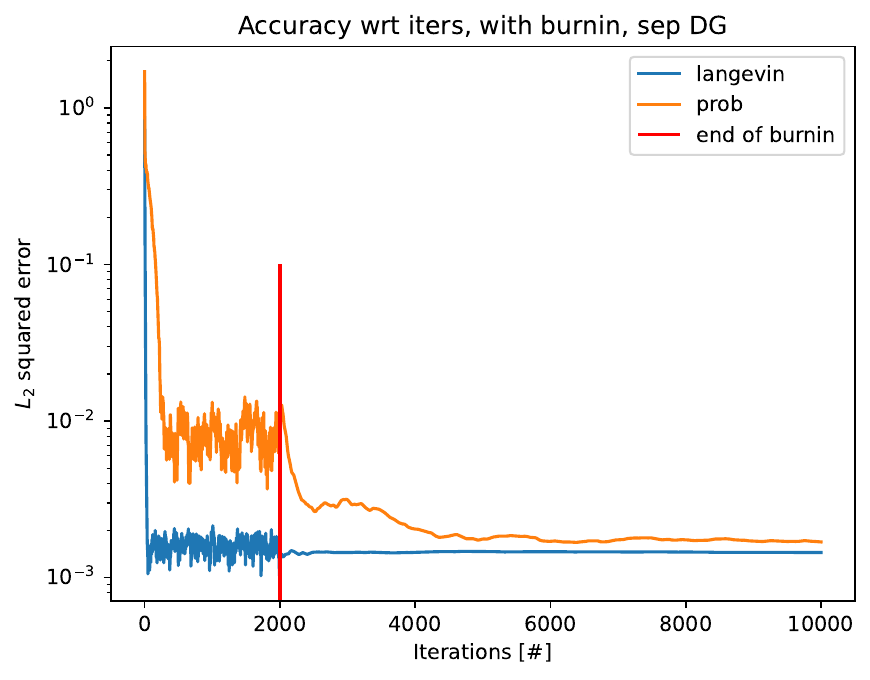
\includegraphics[width=\textwidth]{figures/experiments/baseline/iters_acc_comp_iters_no_avg_sep.png}
        \caption{Separate qubit}
        \label{fig:conv-plot-sep-DG-sub}
    \end{subfigure}
    \caption{Convergence plot with \nitern{10000} and \nburninn{2000} for $n=3$}
    \label{fig:conv-plot}
\end{figure}

As we can see in both these plots, the 2 algorithms achieve the same accuracy, however Projected Langevin converges much faster. This confirms the hypothesis that the gradient is beneficial. It is also a confirmation that both data generation approaches give similar results. The only difference we see is that the convergence of the prob-estimator is faster with the mixed qubit approach, however, this does not change the overall conclusion between the algorithms. Note that, as indicated in the previous section \ref{section:numerical-exp}, we also use the running average for Langevin, which is why it is smoothed out after the end of the burn-in period.

\subsection*{Convergence across ranks}
A second element that we would like to check is how these algorithms perform if the rank $\rho$ is different from 2. These are the results we get for 3 combinations, rank 1, rank 2 and rank $d=8$ using mixed qubit data generation:

\begin{figure}[H]
    \centering
    \begin{subfigure}[b]{0.49\textwidth}
        % experiments/iterations_no_avg_rank1
        \centering
        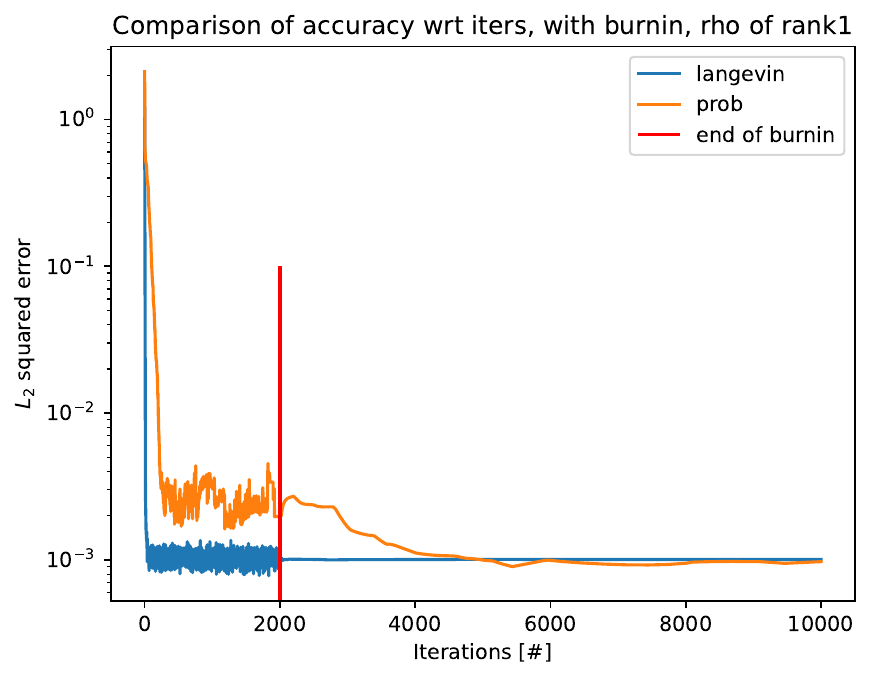
\includegraphics[width=\textwidth]{figures/experiments/baseline/diff_rank/iters_acc_comp_iters_no_avg_rank1-1.png}
        \caption{\rhorankn{d=1}}
        \label{fig:conv-plot-diff-rank-1-sub}
    \end{subfigure}
    \hfill
    \begin{subfigure}[b]{0.49\textwidth}
        % experiments/iterations_no_avg
        \centering
        \includegraphics[width=\textwidth]{figures/experiments/baseline/diff_rank/iters_acc_comp_iters_no_avg-1.png}
        \caption{\rhorankn{d=2}}
        \label{fig:conv-plot-diff-rank-2-sub}
    \end{subfigure}
    \begin{subfigure}[b]{0.49\textwidth}
        % experiments/iterations_no_avg_rankd
        \centering
        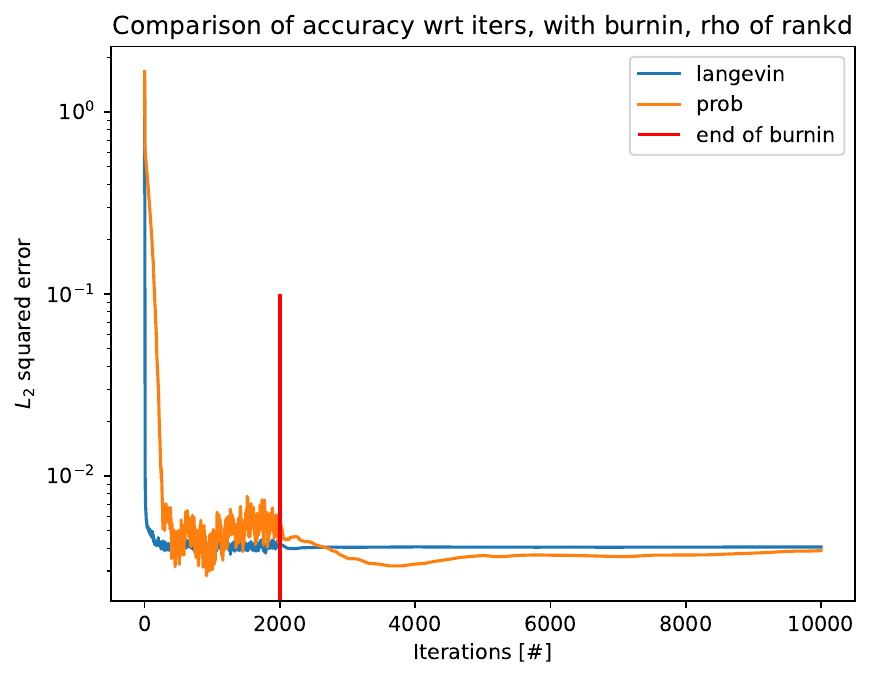
\includegraphics[width=\textwidth]{figures/experiments/baseline/diff_rank/iters_acc_comp_iters_no_avg_rankd-1.png}
        \caption{\rhorankn{d=8}}
        \label{fig:conv-plot-diff-rank-d-sub}
    \end{subfigure}
    \caption{Convergence plot with \nitern{10000} and \nburninn{2000} with \rhorank $\in \{1,2,d=8\}$ for $n=3$  }
    \label{fig:conv-plot-diff-rank}
\end{figure}

We can see that the result is sensibly the same across all ranks, hence confirming our hypothesis that rank 2 is representative of other ranks. It is interesting to note that rank 1 takes longer to converge for the prob-estimator, which means that the density matrix is more difficult to approximate in this situation. This matches our intuition, as a sum of nonzero matrix random samples (forming a Markov chain in this case) is of full rank.

\subsection*{Convergence across qubit count}

A final element that is interesting to compare is how convergence is impacted by the qubit count. In this case, we will be running both algorithms with $n\in\{3,4,5\}$:

\begin{figure}[H]
    \centering
    \begin{subfigure}[b]{0.49\textwidth}
        % experiments/iterations_no_avg_rank1
        \centering
        \includegraphics[width=\textwidth]{figures/experiments/baseline/diff_n_qubits/iters_acc_comp_iters_no_avg-1.png}
        \caption{$n=3$}
        \label{fig:conv-plot-diff-n-3-sub}
    \end{subfigure}
    \hfill
    \begin{subfigure}[b]{0.49\textwidth}
        % experiments/iterations_no_avg_n4
        \centering
        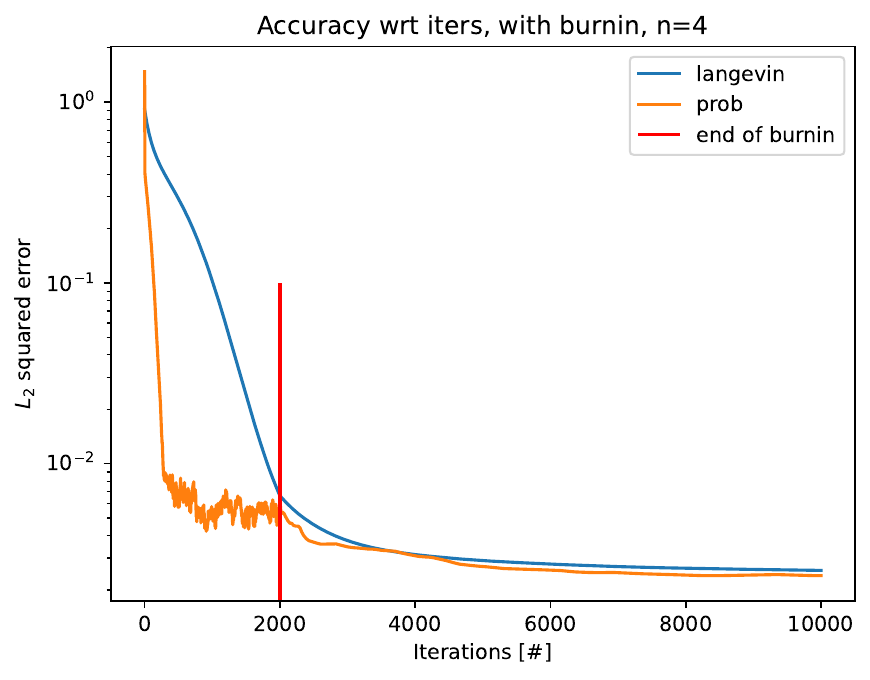
\includegraphics[width=\textwidth]{figures/experiments/baseline/diff_n_qubits/iters_acc_comp_iters_no_avg_n4-1.png}
        \caption{$n=4$}
        \label{fig:conv-plot-diff-n-4-sub}
    \end{subfigure}
    \begin{subfigure}[b]{0.49\textwidth}
        % experiments/iterations_no_avg_n5
        \centering
        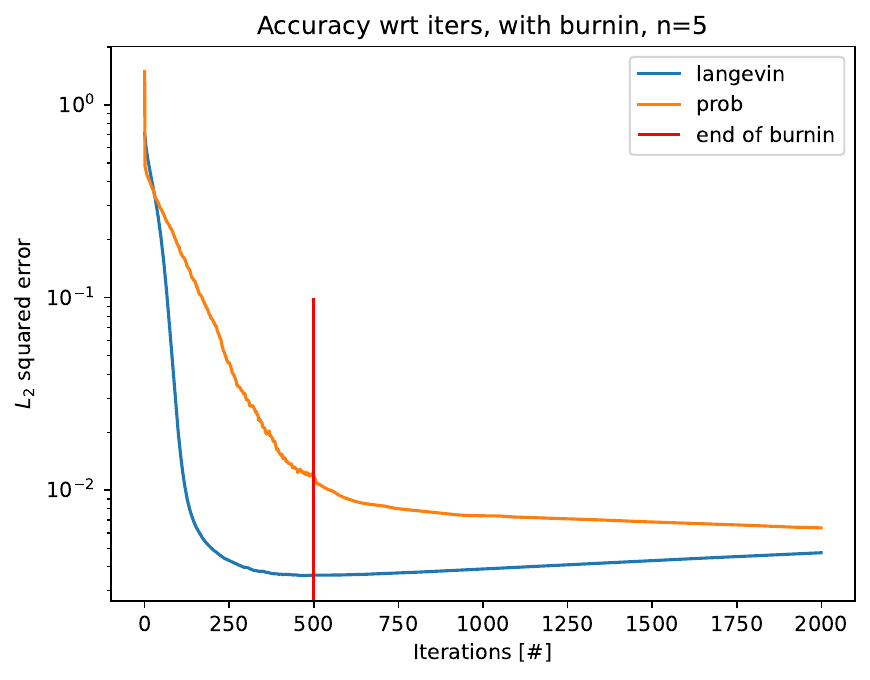
\includegraphics[width=\textwidth]{figures/experiments/baseline/diff_n_qubits/iters_acc_comp_iters_no_avg_n5-1.png}
        \caption{$n=5$}
        \label{fig:conv-plot-diff-n-5-sub}
    \end{subfigure}
    \caption{Convergence plot with \nitern{10000} and \nburninn{2000} with $n\in{3,4,5}$}
    \label{fig:conv-plot-diff-n}
\end{figure}

With each qubit increase, we can see that convergence becomes more and more challenging. We also see that for $n=5$, the prob-estimator converges to a higher accuracy than Langevin (for this number of iterations at least). For $n\in\{4,5\}$, we decreased $\eta$ to $0.0001/m$ as otherwise Langevin was not converging. This also explains why this curve is smooth during the burn-in period, as the steps we take are very small (on the order of $1\text{e-}7$). There seems to be a major trade-off appearing for Langevin: either we reduce the step size in order to obtain convergence and accuracy, but pay with convergence time (in iterations), or converge faster, but without being as accurate, or even without obtaining convergence. \medbreak

One important aspect this conclusion however omits is the computation time (in seconds). If we look at the same figures from above \ref{fig:conv-plot-diff-n}, but instead plot the accuracy with respect to time, this is what we obtain:

\begin{figure}[H]
    \centering
    \begin{subfigure}[b]{0.49\textwidth}
        % experiments/iterations_no_avg_rank1
        \centering
        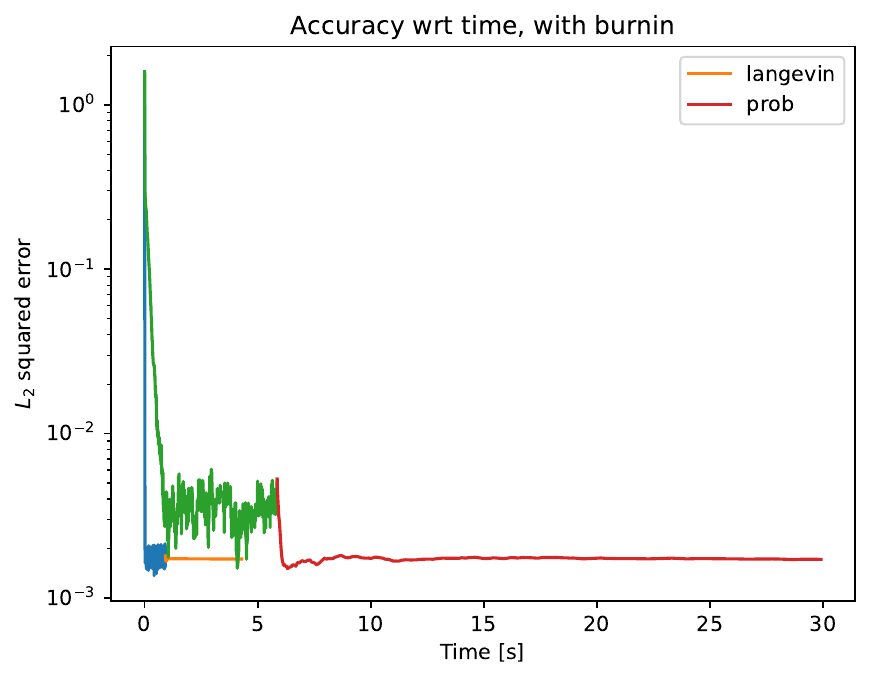
\includegraphics[width=\textwidth]{figures/experiments/baseline/diff_n_qubits/iters_acc_comp_time_no_avg-1.png}
        \caption{$n=3$}
        \label{fig:conv-plot-time-diff-n-3-sub}
    \end{subfigure}
    \hfill
    \begin{subfigure}[b]{0.49\textwidth}
        % experiments/iterations_no_avg_n4
        \centering
        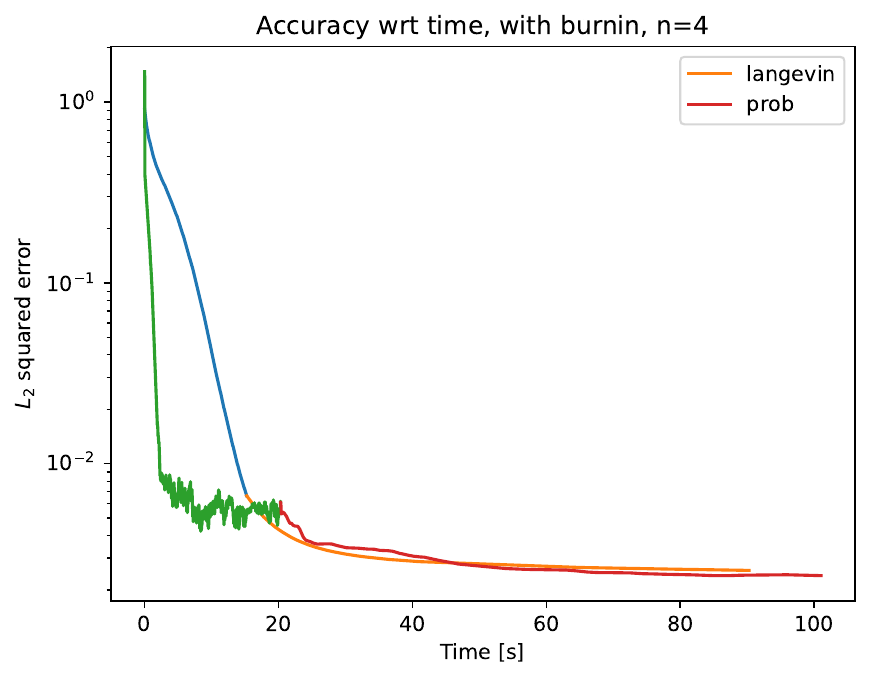
\includegraphics[width=\textwidth]{figures/experiments/baseline/diff_n_qubits/iters_acc_comp_time_no_avg_n4-1.png}
        \caption{$n=4$}
        \label{fig:conv-plot-time-diff-n-4-sub}
    \end{subfigure}
    \begin{subfigure}[b]{0.49\textwidth}
        % experiments/iterations_no_avg_n5
        \centering
        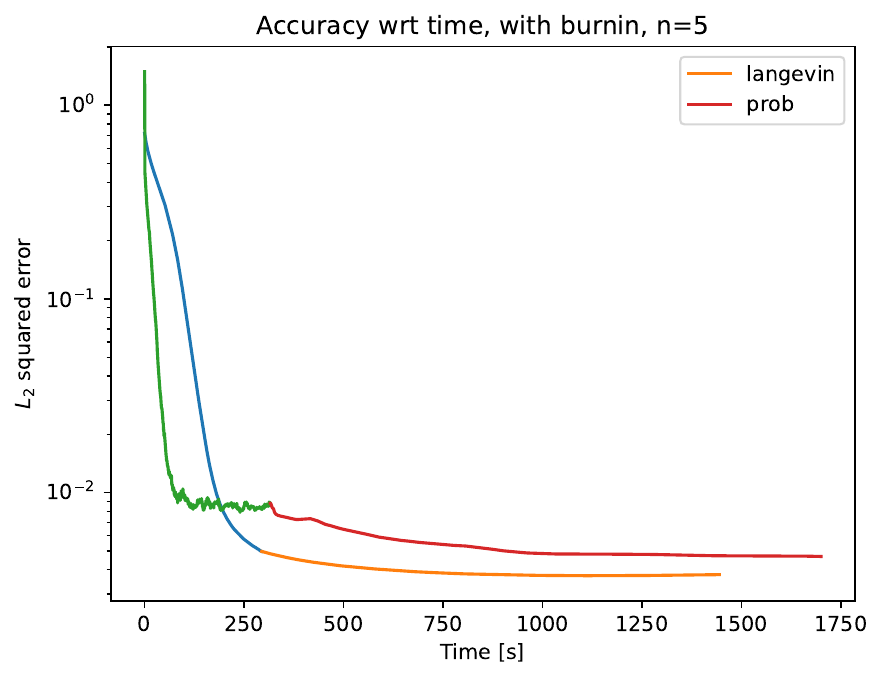
\includegraphics[width=\textwidth]{figures/experiments/baseline/diff_n_qubits/iters_acc_comp_time_no_avg_n5-1.png}
        \caption{$n=5$}
        \label{fig:conv-plot-time-diff-n-5-sub}
    \end{subfigure}
    \caption{Convergence plot with respect to cumulative computation time with \nitern{10000} and \nburninn{2000} with $n\in{3,4,5}$}
    \label{fig:conv-plot-time-diff-n}
\end{figure}

We can see that increasing $n$ and decreasing $\eta$ for Langevin leads to higher computation time for convergence. This is a surprising result, as one might expect Langevin to keep performing consistently better than Metropolis-Hastings when the dimensionality increases. It relates to the original trade-off for Langevin sampling discussed in section \ref{section:ula}: the computation of the gradient should not come at the expense of the convergence time. Here, however, this is what happens: when we increase $n$, the gradient becomes expensive to calculate \textit{and} the number of iterations for the algorithm to converge becomes higher, as we are required to reduce $\eta$. The main cost probably comes from the matrix inversion, although this has not been tested. Note that it is possible that with a better choice of parameters $\theta,\lambda,\beta$ the convergence time (in iterations) would decrease, however it is mostly unlikely given the extent to which it takes time and that the parameters used here were chosen through grid search. More experiments with different combinations of parameters but also larger $n$ would be needed to give a definite answer.\medbreak

These results hint us at the potential advantages of Langevin: it is a method that remains precise when $n$ grows if we keep $\eta$ small enough, however at the expense of computation time. The prob-estimator on the other hand seems to be consistently slow and relatively precise, but without needing any adjustments to a step size parameter. Note that it also remains untested how the same experiment would perform in case of a reduced burn-in duration for the prob-estimator, as given results from section \ref{section:comp-burnin}, the final accuracy seems to be the same across varying burn-in periods. It might be possible for it to converge much faster, even with \nburninn{500} (for $n=3$ at least).\medbreak

Another interesting question to ask in this context is if Langevin is suitable for larger $n$, as one might expect no convergence happening with a very small $\eta$ (if we suppose that the trend of decreasing it is needed). This of course also requires more experiments to be confirmed.

\section{Impact of burn-in duration}\label{section:comp-burnin}
So far, we have settled on using \nburninn{2000} for the burn-in duration with a large number of iterations \nitern{10000}. An interesting question to ask ourselves in this situation is to which degree this value determines the convergence speed, and whether in general convergence will happen if, for example, we reduce \nburnin. For this experiment, we fix \nitern{10000} but we vary \nburnin from $100$ to $6000$. Here are the results we obtained (with mixed qubit data generation):

\begin{figure}[H]
    \centering
    \begin{subfigure}[b]{0.49\textwidth}
        % experiments/burnin_no_avg
        \centering
        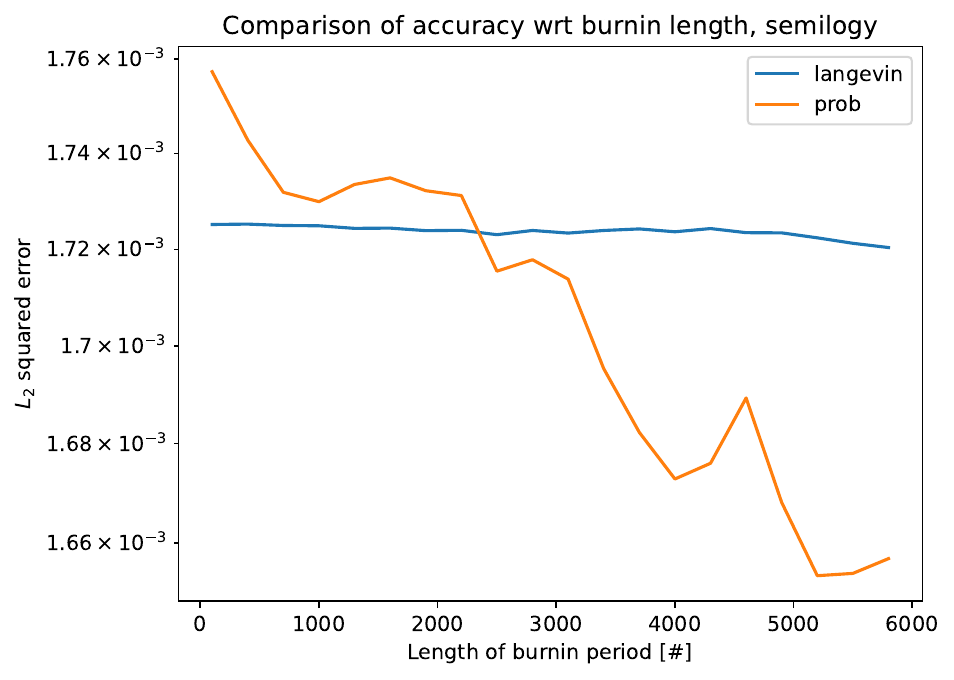
\includegraphics[width=\textwidth]{figures/experiments/burnin/burnin_acc_comp_burnin-1.png}
        \caption{Mixed qubit}
        \label{fig:burnin-comp-mixed-DG-sub}
    \end{subfigure}
    \hfill
    \begin{subfigure}[b]{0.49\textwidth}
        % experiments/burnin_no_avg_sep
        \centering
        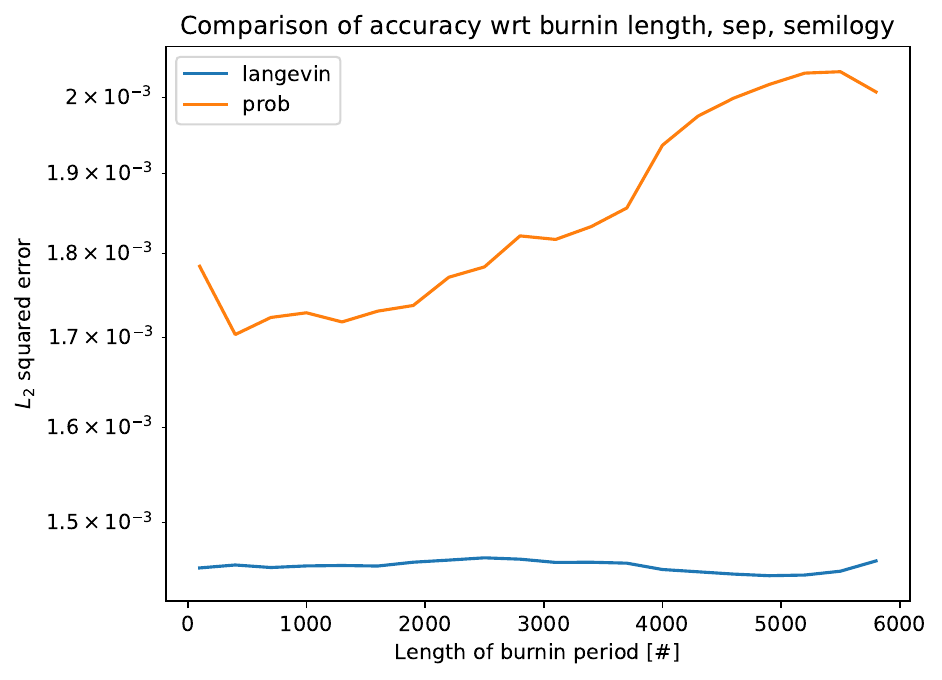
\includegraphics[width=\textwidth]{figures/experiments/burnin/burnin_acc_comp_burnin_sep-1.png}
        \caption{Separate qubit}
        \label{fig:burnin-comp-sep-DG-sub}
    \end{subfigure}
    \caption{Impact of the iterations used for burn-in on the error with $n=3$ and \nitern{10000} fixed}
    \label{fig:burnin-comp}
\end{figure}
The duration of the burn-in very marginally impacts the final accuracy, as it stays on the same order of magnitude of $1\text{e-}3$. There is more variation for the prob-estimator, however, this is a result we could have expected, as Projected Langevin converges very fast, while the prob-estimator takes time.

\section{Impact of number of shots}\label{section:comp-nb-shots}

As discussed in section \ref{section:numerical-exp}, the value of $m=2000$ for the number of shots was chosen as it was the number provided in the original source code for both algorithms. One however might ask how this value impacts the accuracy, as the number of shots is very information-dense: performing the measurement on a system many times (or more exactly replicating the system and measuring the clones) provides better estimates for the empirical probabilities $\hat p_{\mb a, \mb s}$. A priori, we expect that for any algorithm, increasing the number of shots will increase the accuracy. In this experiment, we will be increasing $m$ exponentially from $1\text{e}2$ to $1\text{e}7$, to replicate an experiment from the Langevin paper \cite{meth:bayesian:Langevin:ACMT2024}. The number of iterations, as well as the burn-in duration were reduced to \nitern{5000} and \nburninn{1000}.

\begin{figure}[H]
    \centering
    \begin{subfigure}[b]{0.49\textwidth}
        % experiments/shots
        \centering
        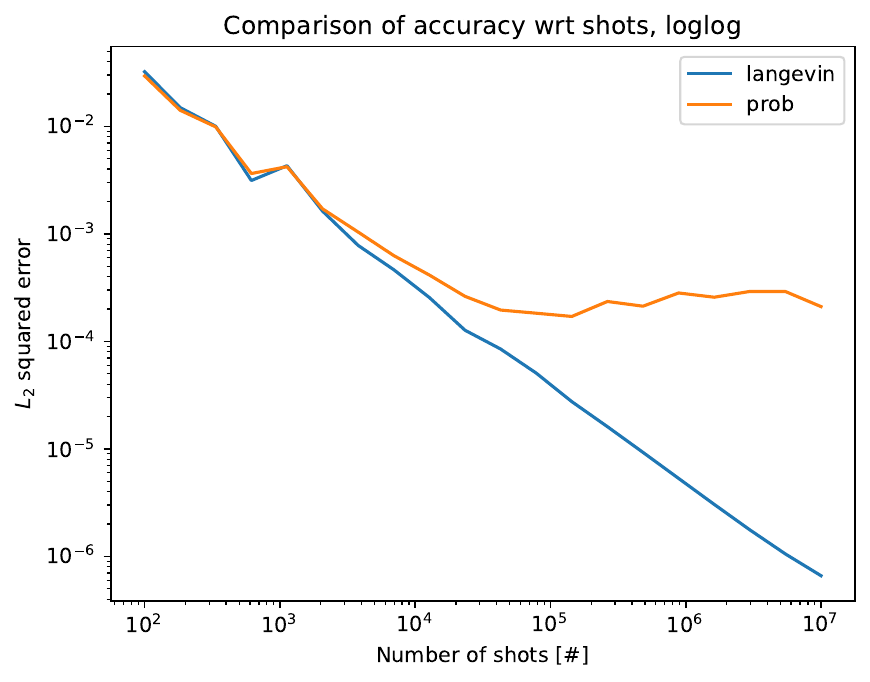
\includegraphics[width=\textwidth]{figures/experiments/shots/shots_acc_comp_shots_exp_loglog-1.png}
        \caption{Mixed qubit}
        \label{fig:shots-comp-mixed-sub}
    \end{subfigure}
    \hfill
    \begin{subfigure}[b]{0.49\textwidth}
        % experiments/shots_sep
        \centering
        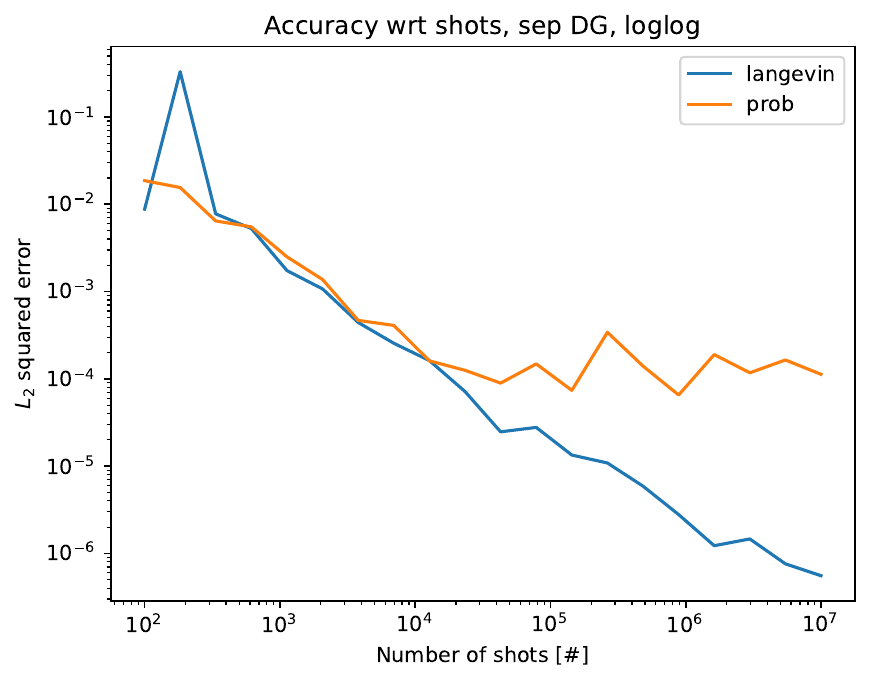
\includegraphics[width=\textwidth]{figures/experiments/shots/shots_acc_comp_shots_exp_sep_loglog-1.png}
        \caption{Separate qubit}
        \label{fig:shots-comp-sep-sub}
    \end{subfigure}
    \caption{Impact of the number of used shots on the error with $n=3$}
    \label{fig:shots-comp}
\end{figure}
We can see quite a surprising result: while Langevin gets the expected behaviour of scaling linearly in the loglog plot, the prob-estimator does not improve beyond a certain threshold of approximately $1\text{e-}4/1\text{e-}5$ shots. It occurs with both data generation processes, which means that it is not the root of the difference. A possible explanation could be that the $\lambda$ parameter, which depends on the number of shots, makes the likelihood term become very large, with the prior stopping being significant. We have therefore tried changing the value of $\lambda$ to a fixed value across all shots' counts (only for the prob-estimator). This is what we obtained with mixed qubit data generation:

\begin{figure}[H]
    % Comes from experiments/
    \centering
    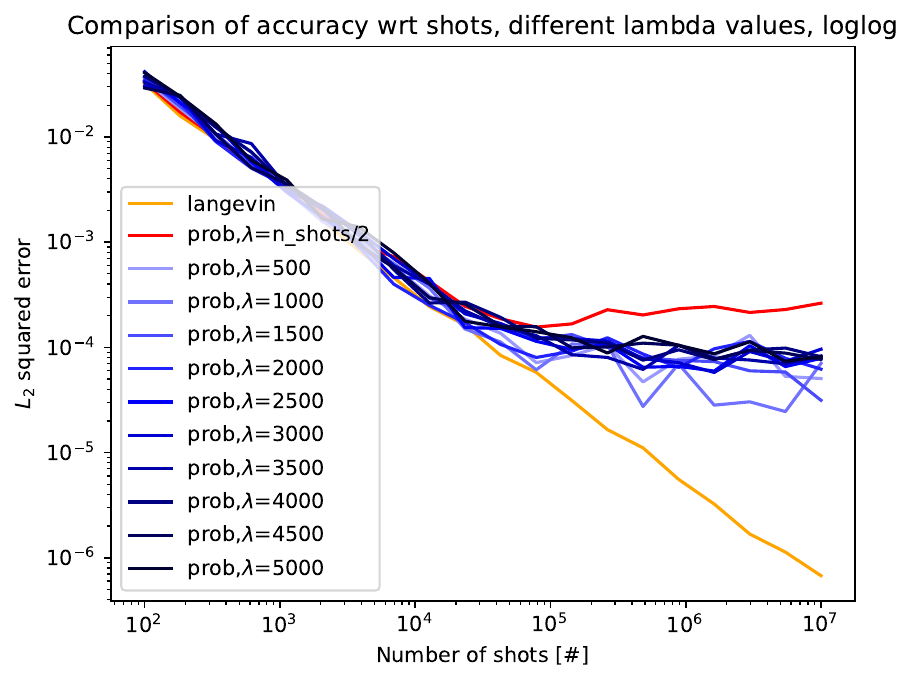
\includegraphics[width=0.7\textwidth]{figures/experiments/shots/shots_acc_comp_shots_exp_lambda_prob_with_var_lambda_loglog-1.png}
    \caption{Impact of the number of used shots on the error with varying parameter $\lambda$ for the prob-estimator with $n=3$}
    \label{fig:shots-comp-prob-var-lambda}
\end{figure}

We can see that even with a fixed $\lambda$ for the prob-estimator, the accuracy stagnates at around $1\text{e-}4$, even for large $m$. We are not exactly sure why this occurs, as we are able to replicate the same behaviour with the original R code (the authors also do not provide metrics beyond $m=2000$ in their paper). The only conclusion we can draw from this result is that it is an inherent property of the method.

\section{Impact of number of measurements}\label{section:comp-nb-meas}
The number of measurements, or observables, is another interesting aspect to explore. While in general, we assume a complete measurement experiment, here we will try to reduce the number of observables to see how both algorithms behave in this setup, and how many observables are needed in order to keep accuracy sufficiently high. Note that inferring the state based on a subset of all measurements is analogous to solving an underdetermined system of equations, and can be seen as compressed sensing. We will be increasing \nmeas from $1$ to either $4^n$ for mixed qubit, or $3^n$ for separate qubit data generation, with the observables randomly chosen at each step. The number of iterations, as well as the burn-in duration, were reduced to \nitern{5000} and \nburninn{1000}. Here is what we obtain:

\begin{figure}[H]
    \centering
    \begin{subfigure}[b]{0.49\textwidth}
        % experiments/meas
        \centering
        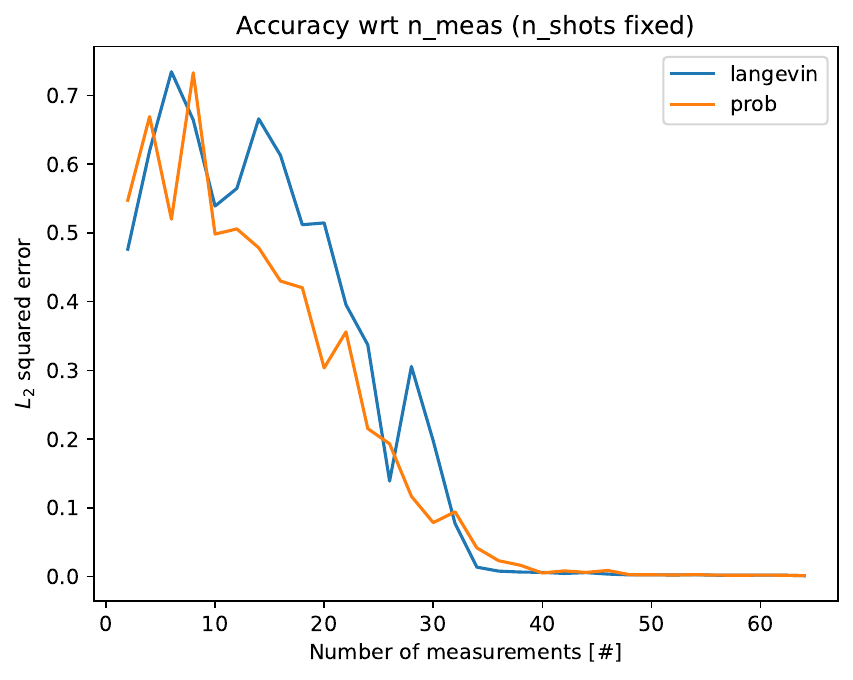
\includegraphics[width=\textwidth]{figures/experiments/meas/meas_acc_comp_meas-1.png}
        \caption{Mixed qubit}
        \label{fig:meas-comp-mixed-sub}
    \end{subfigure}
    \hfill
    \begin{subfigure}[b]{0.49\textwidth}
        % experiments/meas_sep
        \centering
        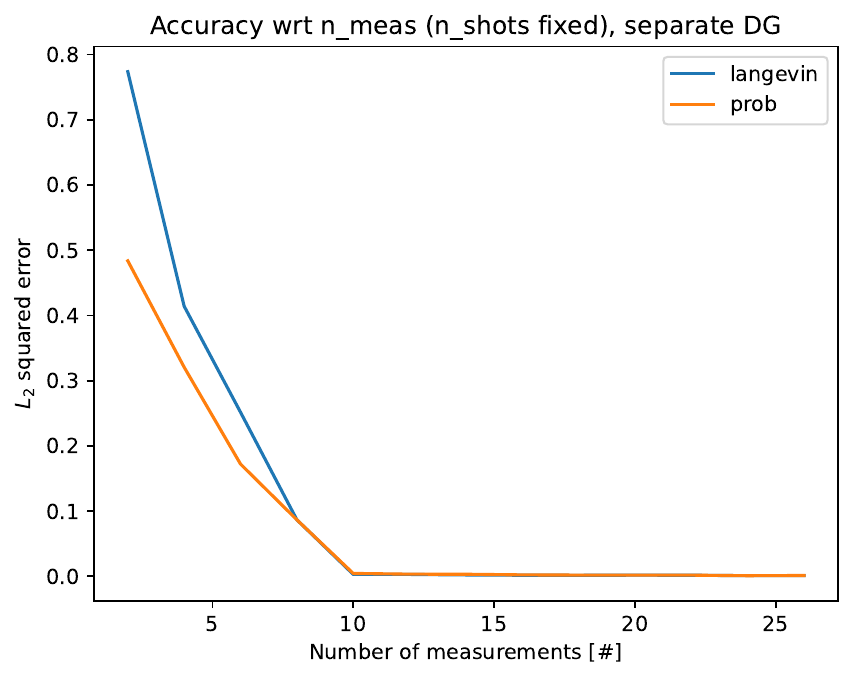
\includegraphics[width=\textwidth]{figures/experiments/meas/meas_acc_comp_meas_sep-1.png}
        \caption{Separate qubit}
        \label{fig:meas-comp-sep-sub}
    \end{subfigure}
    \caption{Impact of the number of used measurements on the error with $n=3$}
    \label{fig:meas-comp}
\end{figure}
We can see that both algorithms perform similarly with both data generation schemas: for mixed qubit, approximately half of the total observables (around 35) are needed to obtain most of the information; for separate qubit, this value seems to be around 10, closer to a third of the total count.\medbreak 

This is not an unexpected result, an approximate approach comes with the downside of being a bit less precise or conveying less information. An interesting plot to obtain related to this one would be the cumulative information gain, which could allow us to answer questions such as ``How many observables do we need in order to be x\% accurate as the equilibrium distribution?'' or ``How many observables do we need in order to have x\% of information of the equilibrium distribution?''.

\section{Impact of knowledge of rank}\label{section:comp-rank-info}
An advantage that the Projected Langevin algorithm has is that it can also incorporate prior information through the Burer-Monteiro factorization, and in particular the rank of the factors. If we know the rank of our true matrix, we can constrain the search space by setting the upper bound of the rank of the sampled matrix $Y$ to be the one of our true matrix $\rho$. One might then ask to which degree this helps. In this experiment, we will be comparing the situation where we have information about the rank, in which case the initial sample for Langevin will be of rank of $\rho$, and otherwise we will keep it fixed as $d=8$. For both cases, we will increase \rhorank from $1$ to $d=8$ to see how accuracy changes, and use mixed qubit data generation. Here are the results:

\begin{figure}[H]
    \centering
    \begin{subfigure}[b]{0.49\textwidth}
        % experiments/rank_known
        \centering
        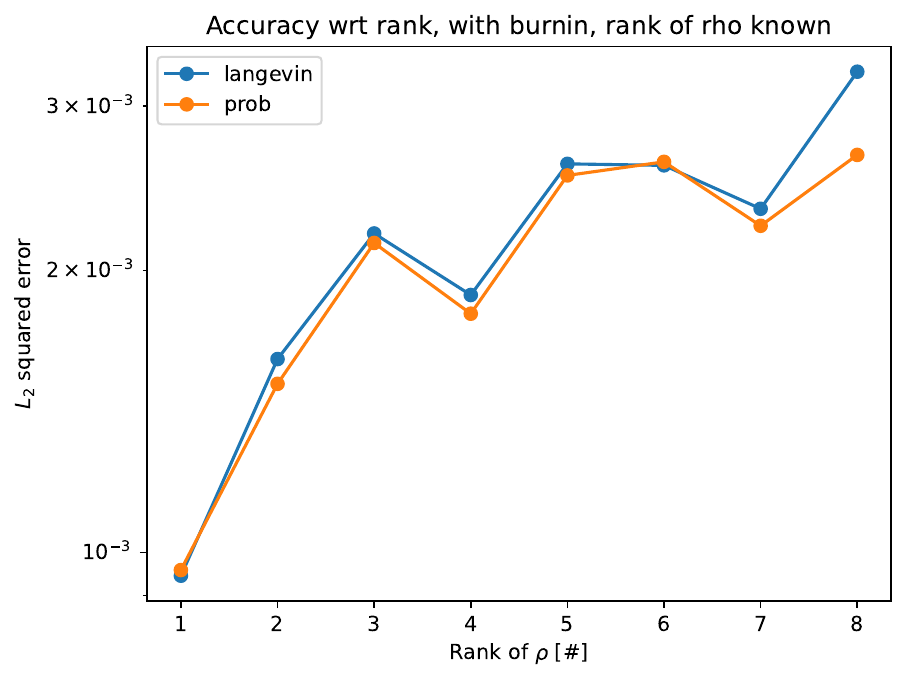
\includegraphics[width=\textwidth]{figures/experiments/rank_info/rank_known-1.png}
        \caption{Rank of $\rho$ known}
        \label{fig:rank-info-sub}
    \end{subfigure}
    \hfill
    \begin{subfigure}[b]{0.49\textwidth}
        % experiments/rank_not_known
        \centering
        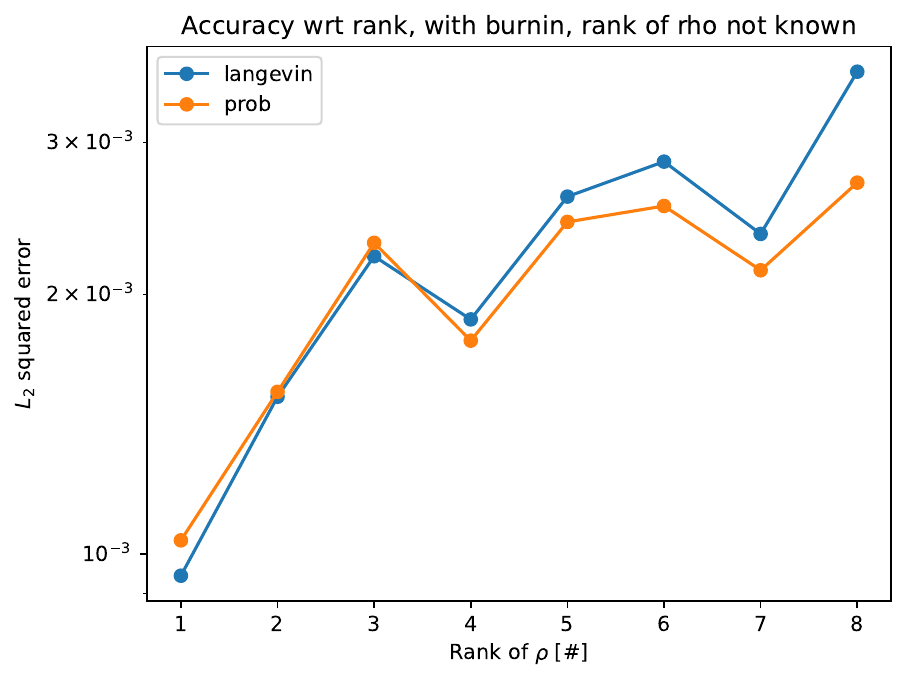
\includegraphics[width=\textwidth]{figures/experiments/rank_info/rank_not_known-1.png}
        \caption{Rank of $\rho$ not known}
        \label{fig:rank-no-info-sub}
    \end{subfigure}
    \caption{Rank knowledge plot for $n=3$}
    \label{fig:rank-info}
\end{figure}

One might also wonder how the parameter $\theta$ in the prior affects this result. In figure \ref{fig:rank-info-var-theta}, we ran the same experiment with $\theta \in \{1\text{e-}6,1\text{e-}3,1\text{e-}2,1\text{e-}1,1\text{e}0, 1\text{e}1\}$:

\begin{figure}[H]
    \centering
    \begin{subfigure}[b]{0.49\textwidth}
        % experiments/rank_known_var_theta_pl
        \centering
        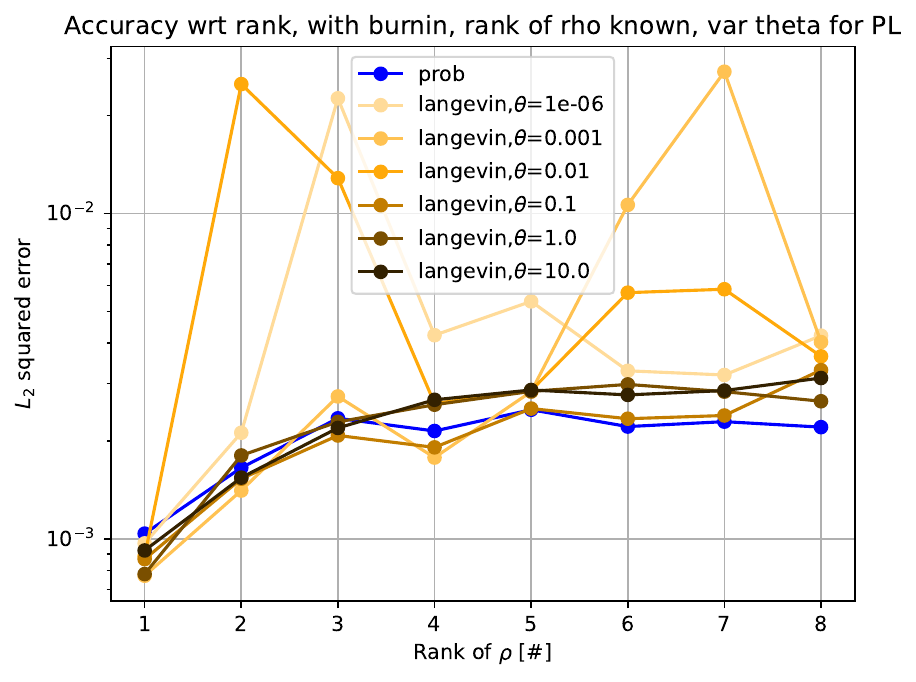
\includegraphics[width=\textwidth]{figures/experiments/rank_info/rank_known_var_theta_pl-1.png}
        \caption{Rank of $\rho$ known}
        \label{fig:rank-info-var-theta-sub}
    \end{subfigure}
    \hfill
    \begin{subfigure}[b]{0.49\textwidth}
        % experiments/rank_not_known_var_theta_pl
        \centering
        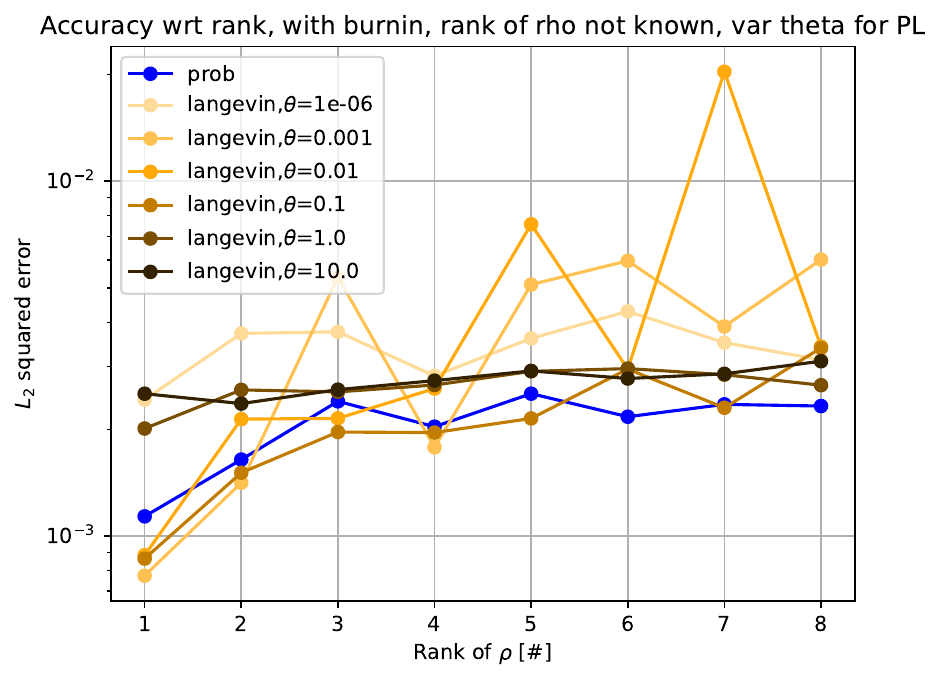
\includegraphics[width=\textwidth]{figures/experiments/rank_info/rank_not_known_var_theta_pl-1.png}
        \caption{Rank of $\rho$ not known}
        \label{fig:rank-no-info-var-theta-sub}
    \end{subfigure}
    \caption{Rank knowledge plot for $n=3$ and different combinations of $\theta$}
    \label{fig:rank-info-var-theta}
\end{figure}

We can also try this experiment for $n=4$ (hence from \rhorankn{1} to \rhorankn{d=16}), to see if it generalizes to higher qubit counts:
\begin{figure}[H]
    \centering
    \begin{subfigure}[b]{0.49\textwidth}
        % experiments/rank_known_n4
        \centering
        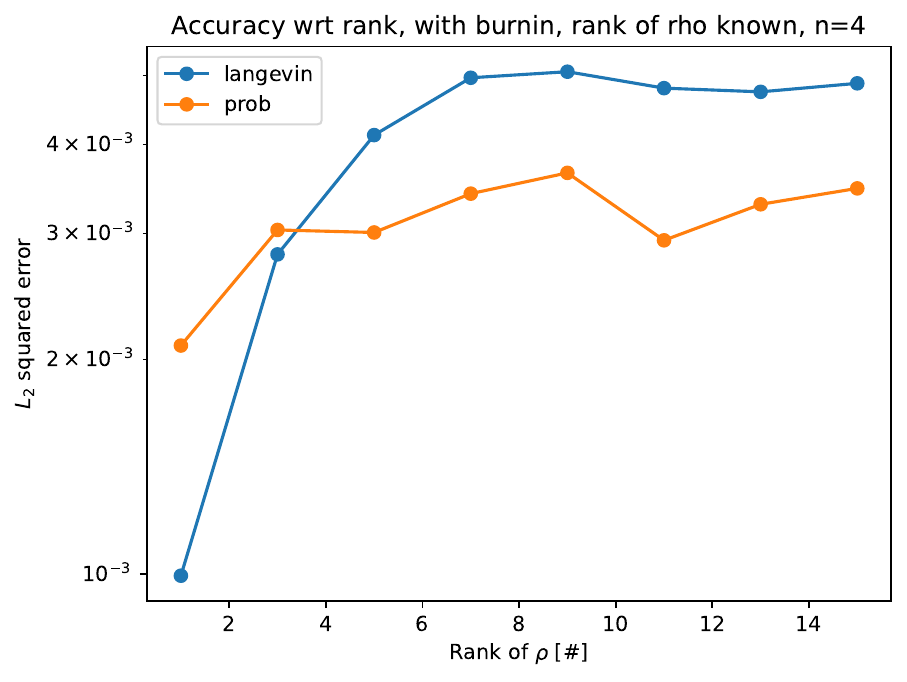
\includegraphics[width=\textwidth]{figures/experiments/rank_info/rank_known_n4-1.png}
        \caption{Rank of $\rho$ known}
        \label{fig:rank-info-n4-sub}
    \end{subfigure}
    \hfill
    \begin{subfigure}[b]{0.49\textwidth}
        % experiments/rank_not_known_n4
        \centering
        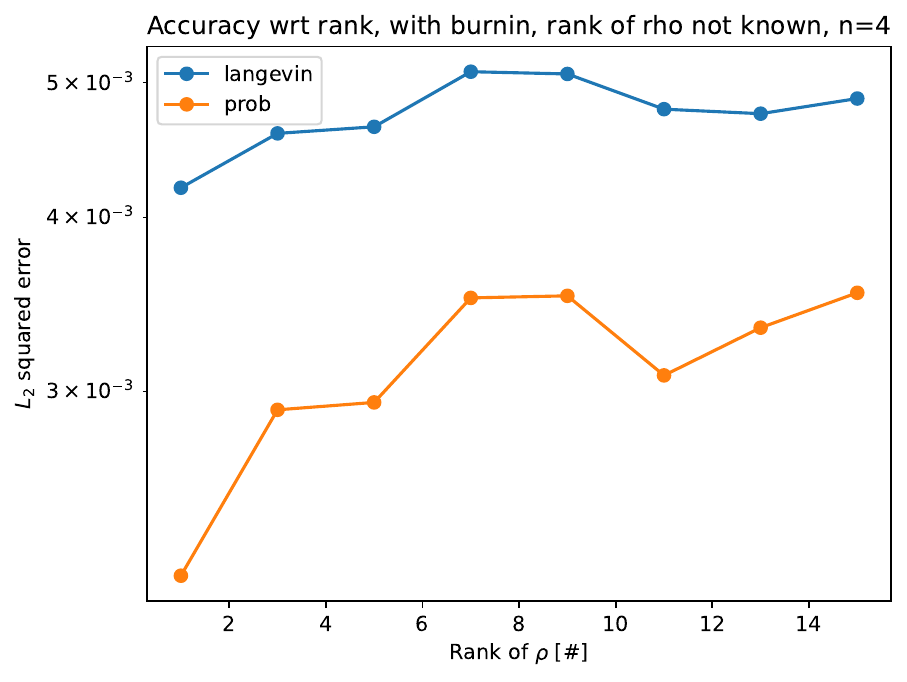
\includegraphics[width=\textwidth]{figures/experiments/rank_info/rank_not_known_n4-1.png}
        \caption{Rank of $\rho$ not known}
        \label{fig:rank-no-info-n4-sub}
    \end{subfigure}
    \caption{Rank knowledge plot for $n=4$}
    \label{fig:rank-info-n4}
\end{figure}

These results are surprising, as they show that the information about the rank only leads to a marginal improvement in accuracy (it stays on the same order of magnitude). The most insightful plot is figure \ref{fig:rank-info-var-theta} with the different combinations of $\theta$: we see on the left figure \ref{fig:rank-info-var-theta-sub}, where we known the rank, that the error increases for \rhorank{$\in \{1,2,3\}$} and stabilizes for other ranks around $2\text{e-}3/3\text{e-}3$ (with more variance for smaller $\theta$). On the right figure \ref{fig:rank-no-info-var-theta-sub}, some parameters have the same curve, but others, in particular, $\theta \in\{1,10\}$, have a flat curve, with little variation between ranks. The overall conclusion remains however the same regardless of the parameter value: the information gain is minimal and the error is of the same order of magnitude.
These results seems to generalize for higher $n$, as we see on figure \ref{fig:rank-info-n4}. \medbreak

There are 2 possible conclusions we can draw from this: either the upper bound that the factorization brings plays a small role in how it constrains the search space (with the prior and its parameters having much more impact), however, it is also possible that the way we obtain our first sample is not correct, and even though samples are numerically of different rank, they tend to be too similar (see the appendix \ref{section:init-sample-gen} for more details on how the first sample is generated). More experiments are needed to investigate these results.\medbreak

Another interesting insight we can draw from figures \ref{fig:rank-info}, \ref{fig:rank-info-var-theta} and \ref{fig:rank-info-n4} (for both cases, whether we know the rank of $\rho$ or not) is that approximating matrices of high rank tends to be more difficult. It is not clear if this is only linked to the fact that we use a low-rank prior, or simply a property of these matrices. Future work could explore non-low-rank priors in the experiments we propose, which would allow to estimate the usefulness of low-rank priors.

\section{Summary}
The previous experiments allow us to conclude several elements about the difference between the prob-estimator and Projected Langevin. \medbreak

First, we can indeed confirm the hypothesis that Langevin converges faster for $n=3$ thanks to the gradient information based on the results we saw in section \ref{section:convergence-comparison}. This algorithm also seems to be more precise for larger $n$, as shown in figure \ref{fig:conv-plot-diff-n-5-sub}. This algorithm however does not seem to scale when the dimensionality increases, as the computational time becomes nearly equivalent to that of the prob-estimator, due to the small $\eta$ needed in order to converge and the high cost of a gradient calculation. This asks the question whether it makes sense to use Langevin in practical applications where $n$ is large. These conclusions seem to be consistent across the data generation processes, as we saw in figure \ref{fig:conv-plot}, as well as ranks (figure \ref{fig:conv-plot-diff-rank}).\medbreak

Second, for both algorithms, any burn-in duration produces the same accuracy for $n=3$, assuming the total iteration count is sufficiently large (\nitern{10000} in this case). As we see in figure \ref{fig:burnin-comp}, from \nburninn{100} to \nburninn{6000}, the curves stays close to flat.\medbreak

Third, Projected Langevin scales when the number of shots increases, while the prob-estimator does not beyond a threshold. As we saw in section \ref{section:comp-nb-shots}, the prob-estimator does not get more accurate after approximately $1\text{e-}4/1\text{e-}5$ shots, while Langevin has a straight line in the log-log plot of figure \ref{fig:shots-comp}. This is further confirmed in figure \ref{fig:shots-comp-prob-var-lambda}, where $\lambda$ is fixed (not depending on $m$) and tested with different values for the prob-estimator. This means that the prob-estimator is not suitable for obtaining high precision estimates of $\rho$ in situations when a large number of shots is available.\medbreak

Fourth, the number of measurements or observables needed in order to stay accurate is the same for both Projected Langevin and the prob-estimator. Indeed, the data generation process has much more importance, and we observe mixed qubit needing on average half of the total number, while separate qubit only a third, as visible in figure \ref{fig:meas-comp}. This confirms our intuition that an exact method needs fewer observables than an approximate method.\medbreak

Finally, for Projected Langevin, knowing the true rank of $\rho$ only leads to marginally better accuracy. Indeed, figures \ref{fig:rank-info}, \ref{fig:rank-info-var-theta} and \ref{fig:rank-info-n4} all result in the same conclusion: the rank of $\rho$ has more importance on the accuracy than having information about it.

\chapter{Algorithm vs prior: what matters the most?}\label{section:algo-vs-prior}
The previous experiments in Chapter \ref{section:numerical-exp} showed us that for a small number of qubits $n$, Projected Langevin tends to converge faster in terms of iterations. This raises the question of ``why'', as \cite{meth:bayesian:Langevin:ACMT2024} not only brings a new algorithm, but also a new prior. In this chapter, we will introduce 2 new algorithms, Metropolis-Hastings with Student-t prior (MHS) and Metropolis-Hastings with Gibbs with Student-t prior (MHGS) in order to try to understand which part contributes most. By combining Metropolis-Hastings from the prob-estimator with the Student-t prior from Projected Langevin, we can estimate whether the prior is a silver bullet that can solve Bayesian Quantum Tomography, or if Langevin is still a mandatory component for it to work.\medbreak

This chapter is the second main contribution of this thesis and is structured as follows: in \ref{section:mhs-and-mhgs} we will describe in detail both algorithms, then in \ref{section:proposal-choice} we will talk about the choice of the proposal and finally in \ref{section:mhs-mhgs-num-exp} we will numerically evaluate how these algorithms perform.
\section{Introducing new algorithms: MHS and MHGS}\label{section:mhs-and-mhgs}
\subsection*{Metropolis-Hastings with Student-t prior}
\textit{Metropolis-Hastings with Student-t} (MHS), as its name suggests, is a Metropolis-Hastings-based algorithm. It is a vanilla version of the original algorithm, as the modifications are minor. The main difference comes from the fact that we work directly on the matrix space, rather than vectors or scalars. More precisely, we utilize the Burer-Monteiro factorization from the Projected Langevin approach (as seen in section \ref{section:projected-langevin}) to work directly with $Y \in \mathbb{R}^{2d \times 2r}$, where we do the reverse isomorphic transformation $\psi^{-1}$ to map back to $Y \in \mathbb{C}^{d\times r}$ to calculate $\hat \rho$. We also use the spectral scaled Student-t prior from Langevin (defined on $\mathbb{C}$ here):
\begin{equation}
    \nu_{\theta} (Y) = C_\theta \det(\theta^2I_d + YY^\dagger)^{-(2d+r+2)/2}
\end{equation}
When converted to the real domain, this results in the same posterior as in Projected Langevin $\hat \mu_{\lambda, \theta}(\tilde Y, \mb D) =\exp(-\tilde f_{\lambda, \theta}(\tilde Y, \mb D))$, where 
\begin{equation}
    \tilde f_{\lambda, \theta}(Y, \mb D) = \lambda \sum^{M}_{i=1} (\hat p_m - \sqrt{2}\tr(\tilde A_m \tilde Y \tilde Y^{T}))^2 + \cfrac{2d + r + 2}{4}\log \det(\cfrac{\theta^2}{\sqrt 2}I_{2d} + \sqrt 2 \tilde Y \tilde Y^{T}) + \tilde C
\end{equation}
In practice, we also the log-transformation trick as described in section \ref{section:Metropolis-Hastings} because it allows for better numerical stability. Assuming a proposal $p_1(\tilde Y|\tilde Y^{(k-1)})$ (which we will describe in more detail in the next section \ref{section:proposal-choice}) and acceptance rate $A_1$, the pseudocode for the resulting algorithm is the following:\medbreak

\begin{algorithm}[H]
    \DontPrintSemicolon
    \SetKwInOut{Input}{Input}
    \SetKwInOut{Output}{Output}

    %\underline{Prob-estimator}\;
    \Input{$T \in \mathbb{N}, Y^{(0)} \in \mathbb{C}^{d \times r}, \theta \in \mathbb{R}, \lambda \in \mathbb{R}$}
    \Output{$\tilde Y \in \mathbb{R}^{2d\times 2r}$}
    $\tilde Y^{(0)} \gets \psi(Y^{(0)})$\;
    $\tilde Y = \mb 0$\;
    \For{$k\gets 1:T$}{
        Sample $\tilde Y^* \sim p_1(\tilde Y|\tilde Y^{(k-1)})$\;
        Sample $u \sim U(0, 1)$\;
        $\alpha \gets \min\left\{\log A_1(\tilde Y^*, \tilde Y^{(k-1)}, \theta, \lambda), \log(1)\right\}$\;
        \eIf{$\log(u) \leq \alpha$}{
            \tcp*[l]{Accept $\tilde Y^*$}
            $\tilde Y^{(k)} \gets \tilde Y^*$
        }{
            \tcp*[l]{Reject $\tilde Y^*$}
            $\tilde Y^{(k)} \gets \tilde Y^{(k-1)}$
        }
        $\tilde Y \gets \frac{1}{k} \tilde Y^{(k)} + (1 - \frac{1}{k})\tilde Y$\;
    }
    \caption{Metropolis-Hastings with Student-t prior}
\end{algorithm}\medbreak
where $\lambda$ is a weight parameter for the likelihood, $\theta$ a scale parameter for the prior, $T$ the number of iterations and $Y^{(0)}$ the initial sample.\medbreak


\subsection*{Metropolis-Hastings with Gibbs with Student-t prior}
\textit{Metropolis-Hastings with Gibbs with Student-t prior} (MHGS) is an extension of MHS and is an attempt to imitate more closely the way the prob-estimator works. Indeed as we saw in section \ref{section:prob-estimator}, the prob-estimator resembles more Metropolis-within-Gibbs than pure Metropolis-Hastings, as it iterates over each dimension for each Metropolis-Hastings iteration. With this in mind, MHGS works by sampling each entry of the matrix $\tilde Y \in \mathbb{R}^{2d\times 2r}$ separately. If we assume the proposal $p_2(y|\tilde Y^{(k-1)}_{ij})$ and acceptance rate $A_2$, this results in the following algorithm:\medbreak

\begin{algorithm}[H]
    \DontPrintSemicolon
    \SetKwInOut{Input}{Input}
    \SetKwInOut{Output}{Output}

    %\underline{Prob-estimator}\;
    \Input{$T \in \mathbb{N}, Y^{(0)} \in \mathbb{C}^{d \times r}, \theta \in \mathbb{R}, \lambda \in \mathbb{R}$}
    \Output{$\tilde Y \in \mathbb{R}^{2d\times 2r}$}
    $\tilde Y^{(0)} \gets \psi(Y^{(0)})$\;
    $\tilde Y = \mb 0$\;
    \For{$k\gets 1:T$}{
        $\tilde Y^{(k)} \gets \tilde Y^{(k-1)}$\;
        \For{$i\gets 1:2d$}{
            \For{$j\gets 1:2r$}{
                Sample $y^* \sim p_2(y|\tilde Y^{(k)}_{ij})$\;
                Sample $u \sim U(0, 1)$\;
                $\alpha \gets \min\left\{\log A_2(y^*, \tilde Y^{(k)}_{ij}, \theta, \lambda), \log(1)\right\}$\;
                \eIf{$\log(u) \leq \alpha$}{
                    \tcp*[l]{Accept $y^*$}
                    $\tilde Y^{(k)}_{ij} \gets y^*$
                }{
                    \tcp*[l]{Reject $y^*$}
                    $\tilde Y^{(k)}_{ij} \gets \tilde Y^{(k)}_{ij}$
                }
            }
        }
        $\tilde Y \gets \frac{1}{k} \tilde Y^{(k)} + (1 - \frac{1}{k})\tilde Y$\;
    }
    \caption{Metropolis-Hastings with Gibbs with Student-t prior}
\end{algorithm}\medbreak
where $\lambda$ is a weight parameter for the likelihood, $\theta$ a scale parameter for the prior, $T$ the number of iterations and $Y^{(0)}$ the initial sample.\medbreak

\section{Proposal choice}\label{section:proposal-choice}
A very important element of these approaches is the choice of the proposal. As we are trying to be as close as possible to the prob-estimator for the algorithm part, it is not clear which proposal should be chosen. The original algorithm samples from a prior, be it a Gamma distribution for $\gamma$ or the unit sphere for $V$. Sampling from these distributions is, however, only relevant in the rank-1 factorization that the authors use, and not as a general proposal. Following this logic, we should be sampling from the scaled Student-t distribution, however, it is not obvious how this should be done, with further work required to investigate it. In the following sections, we will discuss the considered options.

\subsection*{Proposal for MHS}
For the MHS algorithm, we considered 3 main options for $p_1(\tilde Y| \tilde Y ^{(k-1)})$: the normal distribution centered at the current sample (which is a very common proposal), the normal distribution centered at 0 (independent normal) and the Gamma distribution, in the same way that is done by the prob-estimator. This last method is not the most appropriate given what we mentioned above, however, we kept it as a point of comparison. We used the adjusted version of the acceptance rate for both the independent normal and the centered normal (note that the proposal component in the numerator and denominator simplify for it, as it is symmetrical), but did not do so for the gamma distribution, as it is not clear how this should be done (even though it is asymmetrical). We summarize them below in \ref{table:proposal-comp-mhs}:
\begin{table}[H]

    \begin{center}
        \begin{tabular}{|c|c|}
            \hline
            Proposal name & Equation\\
            \hline\hline
             & \\[-10pt]
            Normal distribution, centered & $\tilde Y^* \gets \tilde Y^{(k-1)} + \sigma \boldsymbol{\eta} \quad\text{with } \boldsymbol{\eta} \sim N(0,1)^{2d\times 2r}$\\
            Normal distribution, independent & $\tilde Y^* \gets \sigma \boldsymbol{\eta} \quad\text{with } \boldsymbol{\eta} \sim N(0, 1)^{2d \times 2r}$\\
            Gamma distribution, centered & $\tilde Y^* \gets \tilde Y^{(k-1)} \odot \exp (\sigma\boldsymbol{\xi})\quad \text{with } \boldsymbol{\xi} \sim U(-0.5, 0.5)^{2d\times 2r}$\\\hline
        \end{tabular}
\end{center}
\caption{Proposals considered for MHS}
\label{table:proposal-comp-mhs}
\end{table}

After running a grid search with parameters $\sigma\in \{0.001, 0.01, 0.05, 0.1, 0.5, 1, 10\}$ and \nitern{5000}, \nburninn{1000} these are the results we obtain: 

\begin{table}[H]

    \begin{center}
        \begin{tabular}{|c|c|c|}
            \hline
            Proposal name & Parameter value & Error ($L_2^2$)\\
            \hline\hline
            Centered normal& 0.001 & 0.093\\
            Centered normal&0.01  &0.115\\
            Independent normal& 0.05 &0.316\\
            Gamma&0.1  &0.423\\
            Gamma&1.0   &0.449\\\hline
        \end{tabular}
\end{center}
\caption{Grid search results over proposals and their scaling parameters for MHS, top 5 entries sorted by error}
\label{table:proposal-grid-search-mhs}
\end{table}
Given this outcome, we settled on using the centered normal as our proposal with $\sigma=0.001$. Note that this choice of proposal is not the best, and as stated previously, we should ideally be sampling from the Student-t distribution to align with the prob-estimator approach. 

\subsection*{Proposal for MHGS}
For the MHGS algorithm, we decided to remove the independent normal distribution as we deemed it to be less relevant, however, kept the two other methods in their scalar version:

\begin{table}[H]

    \begin{center}
        \begin{tabular}{|c|c|}
            \hline
            Proposal name & Equation\\
            \hline\hline
             & \\[-10pt]
            Normal distribution, centered & $y^* \gets \tilde Y^{(k)}_{ij} + \sigma {\eta} \quad\text{with } \eta \sim N(0,1)$\\
            Gamma distribution, centered & $y^* \gets \tilde Y^{(k)} \exp (\sigma u)\quad \text{with } {u} \sim U(-0.5, 0.5)$\\\hline
        \end{tabular}
\end{center}
\caption{Proposals considered for MHGS}
\label{table:proposal-comp-mhgs}
\end{table}
We then re-ran the same gridsearch with \nitern{1000} and \nburninn{300} to obtain the following results: 

\begin{table}[H]

    \begin{center}
        \begin{tabular}{|c|c|c|}
            \hline
            Proposal name & Parameter value & Error ($L_2^2$)\\
            \hline\hline
            Centered normal& 0.1&0.052\\
            Centered normal& 0.05&0.063\\
            Centered normal& 0.001&0.097\\
            Centered normal& 10.0&0.165\\
            Centered normal& 1.0&0.166\\\hline
        \end{tabular}
\end{center}
\caption{Grid search results over proposals and their scaling parameters for MHGS, top 5 entries sorted by error}
\label{table:proposal-grid-search-mhgs}
\end{table}
As we can see, the centered normal is once again the best result (in this case with standard deviation $\sigma=0.1$), which confirms us that is it good default choice for proposals in MCMC.

\section{Comparison with the prob-estimator and the Projected Langevin algorithm}\label{section:mhs-mhgs-num-exp}
With the proposals being chosen, we can now proceed to compare these 2 new algorithms to the prob-estimator and Projected Langevin. We will be using the convergence plot to assess the performance, using the separate qubit data generation approach in order to avoid any potential bias that might arise with mixed qubit. The parameter values were kept the same as those from the Langevin algorithm, with $\theta=0.1,\lambda=m/2$. Here is what we obtain:\medbreak

\begin{figure}[H]
    \centering
    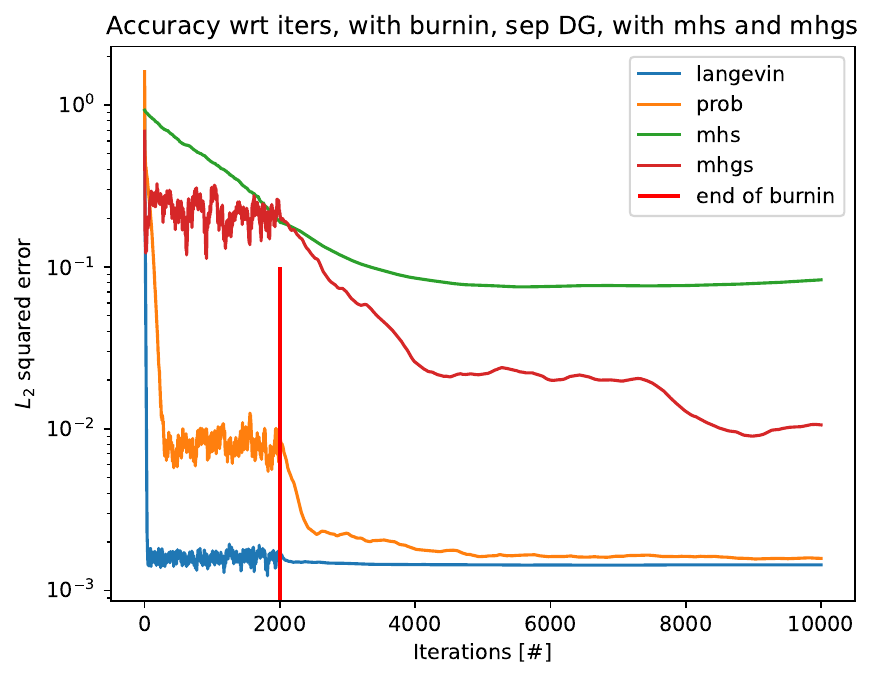
\includegraphics[width=0.7\textwidth]{figures/experiments/mhs_mhgs/iters_acc_comp_iters_no_avg_sep_prob_pl_mhs_mhgs-1.png}
    \caption{Convergence plot with the prob-estimator, Projected Langevin, MHS and MHGS with $n=3$ and separate qubit data generation}
    \label{fig:mhs-mhgs-conv-plot}
\end{figure}


%1) prior in itself is not enough, it must be paired up with a good algorithm
As we can see, both new methods perform worse than the prob-estimator and Projected Langevin, even with a sufficiently good proposal. The MHGS algorithm seems to perform better than MHS, which validates the idea behind the prob-estimator, and other techniques such as \cite{Mai22, LLJL20}, which all sample one-dimensional distributions across dimensions instead of directly sampling from the joint. This however comes at the expense of very long computation times, something that was also visible in section \ref{section:convergence-comparison}, figure \ref{fig:conv-plot-time-diff-n-3-sub}.\medbreak

The major conclusion to draw however from this result is that the prior is not a solution on its own, as pairing it with another algorithm does not lead to better or similar accuracy. The similar results obtained from two different algorithms indicate that it is unlikely to be a coincidence. This of course makes the assumption that the proposal we use is sufficiently good and does not perform suboptimally. This also implies that if a new method is to be implemented using this prior, it is important, after choosing the algorithm well and tuning its hyperparameters, to thoroughly benchmark its performance in order to make sure it is sufficiently accurate. The prior itself does not provide any guarantees on accuracy.\medbreak

The prior also does not help with the convergence speed, as we can see MHGS taking a very long time to converge (and possibly not even converging). This means that Langevin sampling is needed in the context of our comparison. Further work is required to verify if this property comes specifically from Langevin or the gradient information in general, in which case methods such as Hamiltonian Monte Carlo may also be valid.

\chapter{Conclusion and future work}
We have in this master thesis explored how Markov chain Monte Carlo methods can help us solve the Quantum Tomography problem. By leveraging the Bayesian framework, we can include the properties of a density matrix into the prior and approximate the posterior by sampling from it.\medbreak

In particular, we have numerically compared the prob-estimator introduced in \cite{MA17} and the Projected Langevin algorithm introduced in \cite{meth:bayesian:Langevin:ACMT2024} in different experimental settings. Our results in Chapter \ref{section:numerical-exp} demonstrate that 
\begin{itemize}
    \item The Projected Langevin algorithm converges faster than the prob-estimator for $n=3$, however, the computational time becomes a bottleneck with a larger number of qubits. This is due to a need to reduce the stepsize $\eta$ for the algorithm to converge to the equilibrium distribution, and a high cost for the gradient calculation. The Langevin algorithm nevertheless remains more precise for large $n$, making it likely a better choice.
    \item The prob-estimator is not appropriate in situations when a large number of shots is done, for example in order to estimate $\rho$ very precisely. This is due to its bad scaling for large $m$, as demonstrated in figure \ref{fig:shots-comp}. In these situations, the Projected Langevin method seems better suited.
    \item The number of measurements or observables needed in order to estimate $\rho$ to a certain degree of accuracy does not depend on the algorithm, but rather on the data generation process, as seen in section \ref{section:comp-nb-meas}.
    \item For Projected Langevin, knowing the true rank of $\rho$ only leads to marginally better results, as demonstrated in section \ref{section:comp-rank-info}.
\end{itemize}
By then introducing 2 new algorithms in section \ref{section:mhs-and-mhgs}, we wanted to infer what part of the Projected Langevin method, the algorithm or prior, made it perform better. The results conclude that it is probably a combination of both, and the novel low-rank prior by itself is not a silver bullet for Bayesian Quantum Tomography.\medbreak 

This thesis however only explores a subset of the possible experiments, and many questions remain to be answered. We have only compared the prob-estimator and the Projected Langevin algorithm, but as described in the introduction \ref{section:litterature-review}, many other algorithms exist for Bayesian Quantum Tomography. Creating a comprehensive overview of methods with their characteristics would allow researchers to make an informed choice for their use case. It would also be interesting to expand all the experiments that we have done to larger $n$ and test all ranks of $\rho$. \medbreak

We have also talked about convergence in a nonrigorous way, without relying on the convergence bounds that most previous work comes with (including the reference papers). It would be interesting to quantify and compare the obtained numerical results and the expected theoretical bounds.\medbreak

In Chapter \ref{section:algo-vs-prior} we tried to give an answer on why Projected Langevin performs better by proposing 2 new algorithms. The set of experiments we used to draw our conclusion was however very limited and expanding it to the full suite of chapter \ref{section:numerical-exp} would allow to provide more nuance to the answer. The proposed algorithms also form only a small subset of possible priors and algorithms. Exploring other low-rank priors (but also non-low-rank) and algorithms, such as Hamiltonian Monte Carlo for gradient based methods or preconditioned Crank-Nicholson for non-gradient based, would greatly benefit our understanding of the correctness and robustness of our conclusions.

% \bibliographystyle{unsrt}
% \bibliography{bibliography}
\printbibliography

\chapter*{Appendix}
\section*{Derivation of the acceptance rate for the prob-estimator}\label{section:appendix:acc-rate-prob}

\subsection*{Derivation of $\log(R)$}
The first expression $\log(R(\tilde Y, Y^{(t)}, \tilde \gamma, \gamma^{(t)}, V^{(t-1)}, \lambda, \alpha))$ (which we will write as $\log(R(\nu^*, \nu))$) is derived as follows: first, let us define
\begin{align}
    \tilde \ell &= \ell^{}(\sum_{i=1}^{d} \tilde \gamma_i V_i^{(t-1)} (V_i^{(t-1)})^\dagger, \mb D)\\
    \ell^{(t)} &= \ell^{}(\sum_{i=1}^{d} \gamma_i^{(t)} V_i^{(t-1)} (V_i^{(t-1)})^\dagger, \mb D)
\end{align}
In this case of the prob-estimator, we do not have a proposal distribution per se (the sampling from $Gamma(\alpha, 1)$ corresponds to the prior), so the acceptance probability is computed as
\begin{equation}
    R(\nu^*, \nu) = \frac{\pi(\nu^*|D)}{\pi(\nu|D)} = \frac{\exp(-\lambda \tilde\ell) \pi(\nu^*)}{\exp(-\lambda \ell^{(t)})\pi(\nu)}
\end{equation}
The prior $\pi(\nu) = \pi_1(\nu)$ is defined in this case as the Gamma distribution on $Y_i$:
\begin{equation}
    \pi_1(y;\alpha, 1) = \cfrac{1}{\Gamma(\alpha)}y^{\alpha - 1} \exp(-y)
\end{equation}
We can now rewrite $\alpha$ with this definition:
\begin{align}
    R(\nu^*, \nu) = \frac{\exp(-\lambda \tilde\ell) {\tilde Y_i}^{\alpha - 1} \exp(-\tilde Y_i)}{\exp(-\lambda \ell^{(t)}) {Y_i^{(t)}}^{\alpha - 1} \exp(-Y_i^{(t)})}
\end{align}
where we have replaced $y$ by either $\tilde Y_i$ or $Y^{(t)}_i$. Finally, we can apply the log transform:
\begin{align}
    \log(R(\nu^*, \nu)) &= \log\left(\frac{\exp(-\lambda \tilde\ell) {\tilde Y_i}^{\alpha - 1} \exp(-\tilde Y_i)}{\exp(-\lambda \ell^{(t)}) {Y_i^{(t)}}^{\alpha - 1} \exp(-Y_i^{(t)})}\right)\\
    &= \log(\exp(-\lambda \tilde\ell) {\tilde Y_i}^{\alpha - 1} \exp(-\tilde Y_i)) - \log(\exp(-\lambda \ell^{(t)}) {Y_i^{(t)}}^{\alpha - 1} \exp(-Y_i^{(t)}))\\
    &= -\lambda \tilde \ell + (\alpha - 1)\log(\tilde Y_i) - \tilde Y_i - (-\lambda \ell^{(t)} + (\alpha - 1)\log(Y_i^{(t)}) - Y_i^{(t)})\\
    &= -\lambda \tilde \ell + \lambda \ell^{(t)} + (\alpha -1)\log(\frac{\tilde Y_i}{Y_i^{(t)}}) - \tilde Y_i + Y_i^{(t)}
\end{align}

\subsection*{Derivation of $\log(A)$}
The derivation of $\log(A(\tilde V, V^{(t)}, \gamma^{(t)}, \lambda)) = \log(A(\nu^*, \nu))$ is very similar to the one of $\log(R)$, however much simpler since the resulting expression does not involve the prior. The authors do not provide on how the derivation is done, however, the most probable explanation is that the prior is symmetric, hence we can simplify the numerator and denominator. It thus serves a double role of prior \textit{and} proposal. Let's define
\begin{align}
    \tilde \ell &= \ell^{}(\sum_{i=1}^{d} \gamma_i^{(t)} \tilde V_i \tilde V_i^\dagger, \mb D)\\
    \ell^{(t)} &= \ell^{}(\sum_{i=1}^{d} \gamma_i^{(t)} V_i^{(t)} (V_i^{(t)})^\dagger, \mb D)
\end{align}
Then, we can calculate $\log(A)$ as:
\begin{align}
    \log(A(\nu^*, \nu)) &= \log(\frac{\pi(\nu^*)} {\pi(\nu) })\\
                        &= \log(\frac{\exp(-\lambda \tilde \ell)}{\exp(-\lambda \ell^{(t)})})\\
                        &= -\lambda \tilde \ell + \lambda \ell^{(t)}
\end{align}

\subsection*{Generation of the initial sample}\label{section:init-sample-gen}
In order to generate the initial sample $\hat \rho_0 \in \mathbb{C}^{d\times r}$ for MCMC algorithms, we use the following scheme: we start by generating a random unitary matrix $V$ of size $d \times r$, then we generate $\tilde D$ a diagonal matrix, where $\tilde D_{ii} \sim Gamma(1/r, 1)$, which we then normalize and create $D = \sqrt{\tilde D/\sum_{i=1}^{r} \tilde D_{ii}}$. Finally, the generated matrix is calculated as $\hat \rho_0 = V D$. This approach in inspired by what is done in the Langevin code, and seems analogous to what is suggested in \cite{MA17} to generate a rank-1 matrix. In practice, however, the matrix retains its initial rank $r$.
\includepdf[pages={2}]{cover/cover-danila-mokeev.pdf}
\end{document}
